%%%%%%%%%%%%%%%%%%%%%%%%%%%%%%%%%%%%%%%%%%%%%%%%%%%%%%%%%%%%%%%%%%%%%%%%%%
\documentclass[10.5pt,a4j]{jarticle}
%%%%%%%%%%%%%%%%%%%%%%%%%%%%%%%%%%%%%%%%%%%%%%%%%%%%%%%%%%%%%%%%%%%%%%%%%%
\usepackage{amsmath}%数式用*冒頭に書かないとエラーが出るかも
\usepackage[dvipdfmx]{graphicx}% Include figure files
%\usepackage[draft]{graphicx}% Include figure files
\usepackage[dvipdfmx]{color}
%\usepackage{txfonts} %フォントの設定
\usepackage[T1]{fontenc} %フォントの設定
\usepackage{float}%図の挿入
\usepackage{bm}% bold math
\usepackage[top=25truemm,bottom=25truemm,left=25truemm,right=25truemm]{geometry}
%\usepackage{here}
\usepackage{layout}
\usepackage{wrapfig}
\usepackage{indentfirst}
\usepackage{setspace}
\usepackage[]{multicol}
\usepackage{titlesec}
\usepackage[abs]{overpic}
\usepackage{caption}
\usepackage{fancyhdr}
%\usepackage{statex.sty}
%\usepackage{accents.sty}
%\usepackage{comment}
\renewcommand{\abstractname}{}%「概要」を表示しない
\renewcommand{\figurename}{図\,}
%\renewcommand{\thefootnote}{\fnsymbol{footnote}
\pagestyle{fancy}%ページ番号
%\pagestyle{empty}%ページ番号消す
%%%%%%%%%%%%%%%%%%%%%%%%%%%%%%%%%%%%%%%%%%%%%%%%%%%%%%%%%%%%%%%%%%%%%%%%%%
\makeatletter%% プリアンブルで定義する場合は必須

%Define Title, Department and auther%%%%
\def\id#1{\def\@id{#1}}
\def\department#1{\def\@department{#1}}
\def\@maketitle{
\begin{center}
        {\LARGE \@title \\}% 論文のタイトル部分
        \vspace{1.0 zh}
        %\begin{flushright}
        {\large\@department \\}% 所属部分
        %\hspace{1 zw}
        %{\@author \\}% 氏名
        %\end{flushright}
        {\@id}
        \end{center}
        }
 %\def\widebar{\accentset{{\cc@style\underline{\mskip10mu}}}}
%%%%%%%%%%%%%%%%%%%%%%%%%%%%%%%%%%%%%%%%
%%%Setting sections size%%%%%%%%%%%%%%%%
\titleformat*{\section}{\LARGE \bf}
\titleformat*{\subsection}{\Large \bf}
\titleformat*{\subsubsection}{\large \bf}
%%%%%%%%%%%%%%%%%%%%%%%%%%%%%%%%%%%%%%%%

%%%%%%%%%%%%%%%%%%%%%%%%%%%%%%%%%%%%%%%%
\captionsetup[figure]{format=plain, labelformat=simple, labelsep=colon, font=small}
%%%%%%%%%%%%%%%%%%%%%%%%%%%%%%%%%%%%%%%%

%%%%%%%%%%%%%%%%%%%%%%%%%%%%%%%%%%%%%%%%
\newcommand{\bvec}[1]{
\mbox{\boldmath $#1$}
}%BoldMathの定義
{\def\ds{\displaystyle}
%%%%%%%%%%%%%%%%%%%%%%%%%%%%%%%%%%%%%%%%
\setstretch{1.25} % ページ全体の行間を設定
%%%Add section number in Eq.Num%%%%%%%%%
\renewcommand{\theequation}{%
\thesection.\arabic{equation}
}
\@addtoreset{equation}{section}
%%%%%%%%%%%%%%%%%%%%%%%%%%%%%%%%%%%%%%%%

%\setlength{\columnsep}{5 truemm}

\makeatother%% プリアンブルで定義する場合は必須
%%%%%%%%%%%%%%%%%%%%%%%%%%%%%%%%%%%%%%%%%%%%%%%%%%%%%%%%%%%%%%%%%%%%%%%%%%

%%%%%%%%%%%%%%%%%%%%%%%%%%%%%%%%%%%%%
\title{コロイド粒子表面にグラフトした高分子電解質の平衡構造}
\department{移動現象論分野\, 佐脇 航平}
\id{\vspace{-1.25 zh}} %Abstractとの間隔調整
%%%%%%%%%%%%%%%%%%%%%%%%%%%%%%%%%%%%%

\begin{document}
%%%%%%%%%%%%%%%%%%%%%%%%%%%%%%%%%%%%%%%%%%%%%%%%%%%%%%%%%%%%%%%%%%%%%%%%%%
\begin{titlepage}
\begin{center}
\vspace*{50truept}
{\huge 卒業論文(2019年)} \\
\vspace*{100truept}
{\huge コロイド粒子表面にグラフトした\\高分子電解質の平衡構造}\\
\vspace{120truept}
{\LARGE 京都大学工学部工業化学科\\化学プロセスコース}\\
{\LARGE 移動現象論分野}\\
\vspace{50truept}
{\LARGE 佐脇 航平}\\
\vspace{50truept}
\end{center}
\end{titlepage}
%%%%%%%%%%%%%%%%%%%%%%%%%%%%%%%%%%%%%%%%%%%%%%%%%%%%%%%%%%%%%%%%%%%%%%%%%%
%目次の表示
\pagenumbering{arabic}
\tableofcontents
\clearpage

%\maketitle
%%%%%%%%%%%%%%%%%%%%%%%%%%%%%%%%%%%%%

%%%%%%%%%%%%%%%%%%%%%%%%%%%%%%%%%%%%%%%%%%%%%%%%%%%%%%%%%%%%%%%%%%%%%%%%%%

%%%Gaps between text and Eq%%%%%%%%%%
\abovedisplayskip=12 pt
\belowdisplayskip=12 pt
%%%*only use with smsmath%%%%%%%%%%%%
%%%%%%%%%%%%%%%%%%%%%%%%%%%%%%%%%%%%%

%%%%%%%%Text%%%%%%%%%%%%%%%%%%%%%%%%%
%\begin{multicols}{2}
    %\textwidth=22zw
%%%%%%%%%%%%%%%%%%%%%%%%%%%%%%%%%%%%%
\section{緒言}
%%%%%%%%%%%%%%%%%%%%%%%%%%%%%%%%%%%%%
\subsection{研究目的}
%%%%%%%%%%%%%%%%%%%%%%%%%%%%%%%%%%%%%
コロイド材料は,医薬品,セラミック,塗料,顔料などの産業で用いられ,コロイドの分散状態を安定させることは実用的観点から非常に重要性である.安定したコロイド分散状態とは,粒子が沈澱や凝集を起こさず,長期間状態が変化しないものを指す.コロイドの分散安定性を保つ方法として,静電相互作用を用いる方法やコロイド表面に高分子鎖をグラフトする方法がある.ここでグラフトとは,接合や移植などの意味がある.工業材料としては,コロイド表面に高分子鎖をグラフトする方法が実際に用いられている.しかし,コロイドの分散安定性を制御するために用いる高分子鎖の量や長さは多くの場合,経験的なものである.そのため,コロイド表面に高分子鎖をグラフトした際のコロイド間相互作用を調べることが重要と考え,本研究を行うこととした.また,ここでは,コロイド表面にグラフトされた高分子鎖を高分子ブラシと呼ぶこととする.
%%%%%%%%%%%%%%%%%%%%%%%%%%%%%%%%%%%%%
\subsection{研究概要}
%%%%%%%%%%%%%%%%%%%%%%%%%%%%%%%%%%%%%
本研究では,コロイド表面での高分子ブラシの平衡構造を調べるため,自己無撞着場理論を用いて,高分子ブラシの体積分率を計算し,体積分率によって高分子ブラシの平衡構造を表すとした.また,高分子ブラシが高分子電解質である場合も考慮した.過去の研究\cite{paper1}\cite{paper2}では,コロイド半径が高分子ブラシの回転慣性半径よりも十分に大きい場合を想定し,コロイド表面を平坦として計算していたが,本研究では,コロイド半径が高分子ブラシの回転慣性半径と同程度の大きさを持つ場合を考えるため,また,コロイド間相互作用をより適切に考察するため,コロイド表面の曲率を考慮することを考えた.よって,本研究では,主に次のことを行った.\\

1) Bispherical Coordinate Systemを導入

2) グラフト壁面に曲率ある場合とない場合での高分子ブラシ平衡構造の比較

3) 二粒子間距離の関数としての系の自由エネルギーから粒子間相互作用の考察\\

Bispherical Coordinateにより,コロイドが二つある場合での粒子の曲率の考慮を可能とし,コロイドにグラフトした高分子ブラシの平衡構造を調べた.また,コロイド表面の曲率が高分子ブラシのセグメント濃度分布にどのような影響が与えるかを調べ,そして,曲率を考慮すべきコロイド半径と高分子ブラシの回転慣性半径の比の領域を見出した.
%また,コロイド半径$R$,高分子ブラシの回転慣性半径$R_{g}$は,図\,\ref{FIg.1-2-1}で示す通りである.
%\begin{figure}[h]
%\centering
%\includegraphics[width=33mm]{bis_c3.pdf}
%\caption{}
%\label{FIg.1-2-1}
%\end{figure}

%%%%%%%%%%%%%%%%%%%%%%%%%%%%%%%%%%%%%
\newpage
\section{理論及び計算手法}
%%%%%%%%%%%%%%%%%%%%%%%%%%%%%%%%%%%%%
%%%%%%%%%%%%%%%%%%%%%%%%%%%%%%%%%%%%%
\subsection{自己無撞着場理論}
%%%%%%%%%%%%%%%%%%%%%%%%%%%%%%%%%%%%%
溶媒中にコロイド表面に高分子ブラシをグラフトした系における自己無撞着場理論について説明する.
高分子鎖を構成するすべてのモノマーは化学的に同等であり,相互作用は局所的とする.
自己無撞着場理論では,系内に多数存在する高分子鎖をポテンシャル場中に存在する一本の高分子鎖として平均場近似を行う.
ポテンシャル場中に存在する高分子鎖は, 図\,\ref{Fig.2-1-1}\,(a)に示す格子定数$a$のFlory-Huggins格子の上に置かれ,鎖は格子点を結ぶ軌跡として記述される.
高分子鎖は図\,\ref{Fig.2-1-1}\,(b)に示す長さ $ a $ のセグメント$ N $個からなるとする.
高分子鎖に沿う座標として,一方の末端から測った鎖長を全長 $ \it aN $ を用いて無次元化した鎖長 $ s\,(0 \leq s \leq 1) $ を導入する.
%
%
    \begin{figure}[H]
    \begin{tabular}{cc}
            %1
            \begin{minipage}[t]{0.45\hsize}
            \centering
            \begin{overpic}[keepaspectratio,scale=0.325]{Fig/Fig.1/Fig2_FH_lattice.pdf}
                \put(-15,130){(a)}
              \end{overpic}
                \end{minipage} &
            %2
            \begin{minipage}[t]{0.45\hsize}
            \centering
            \begin{overpic}[keepaspectratio,scale=0.6]{Fig/Fig.1/Fig_chain.pdf}
                \put(-20,130){(b)}
              \end{overpic}
                \end{minipage}
                \end{tabular}
                \renewcommand{\baselinestretch}{0.75}
                \caption{(a)\,Flory-Huggins格子上での高分子鎖\,\,\,(b)高分子ブラシの模式図}
                \label{Fig.2-1-1}
                \end{figure}
%
%
ここで,一端がコロイド表面近傍$\bvec{r}_0$でグラフトしており,片末端が$\bvec{r}$に位置する長さ$s$のグラフト鎖が取りうる配位の統計的重率を$ q( \bvec{r},s ) $とすると,あるポテンシャル場$\Omega(\bvec{r})= \omega_{\rm{P}}(\bvec{r})-ep\psi(\bvec{r}) $での,$ q( \bvec{r},s ) $の$s$に関する発展は次の式$ (\ref{eq2-1-1}) $で表される.ここで,$\omega_{\rm{P}}(\bvec{r})$は高分子ブラシが感じるポテンシャルであり,$\psi(\bvec{r})$は電位を表す.
%
%
\begin{equation}
        \label{eq2-1-1}
        \frac{\partial q( \bvec{r},s )}{\partial s}
        =N
        \left(
            \frac{a^2}{6}\Delta-\Omega(\bvec{r})
        \right)
        q( \bvec{r},s )\\
        \end{equation}
%
%
式 $ (\ref{eq2-1-1}) $ は$ q $ を濃度場と読み替えると,ポテンシャル場 $ \Omega(\bvec{r}) $ 中での拡散方程式となっている.
また,位置$  \bvec{r} $ でのセグメントの体積分率 $ \phi_{\rm{P}}( \bvec{r} ) $ は次の式 $ (\ref{eq2-1-2}) $で表される.
%
%
\begin{equation}
\label{eq2-1-2}
\phi_{\rm{P}}( \bvec{r} )=\frac{\sigma_{\rm{P}}SNa^3}{Q_{\rm{P}}}
\int_{0}^{1} q( \bvec{r},s )q^{\dag}( \bvec{r},1-s ) ds
\end{equation}
%
%
        %\label{eq2}
        %C_\alpha=\int_V d{\bvec {r}}
        %\left\{
        %\int_{s^{(\alpha)}_1}^{s^{(\alpha)}_2}  q( \bvec{r},s )q^{\dag}( \bvec{r},1-s ) ds
        %\right\}
    %\end{eqnarray}
%
%
ここで,$\sigma_{\rm{P}}$は高分子のグラフト密度(数面密度),
$S$は高分子がグラフトしている面積,添字$\rm{P}$は高分子ブラシを表す.また,$ q^{\dag}( \bvec{r},s ) $は,$ q( \bvec{r},s )$とは反対側のもう一方の端点から長さ$1-s$で位置 $  \bvec{r} $に到達する自由鎖の統計的重率であり,$ q( \bvec{r},s ) $と同様に次の式 $ (\ref{eq2-1-1}) $から求められる.
%
$ Q_{\rm{P}} $ は規格化定数であり,以下の式$(\ref{eq2-1-4})$で計算される.

\begin{equation}
\label{eq2-1-4}
Q_{\rm{P}}=\frac{1}{V}\int_{V} d{\bvec r}
\int_{0}^{1} q( \bvec{r},s )q^{\dag}( \bvec{r},1-s ) ds
\end{equation}
%
%
この式 $ (\ref{eq2-1-4}) $は,位置 $  \bvec{r} $において高分子鎖が取りうる全ての配位に比例する量を表している.
以上の式 $ (\ref{eq2-1-1}) $から式 $ (\ref{eq2-1-4}) $を用いて,あるポテンシャル場下での系の体積分率は求められる.
%
電位はポアソン方程式である次の式$(\ref{eq2-1-5})$で計算され,イオン密度分布はポアソン・ボルツマン分布に従うとし,式$(\ref{eq2-1-6})$で計算されるとした.誘電率$\varepsilon$は,系では溶媒が多量であるとし$\varepsilon=\varepsilon_{\rm{w}}\varepsilon_{0}$とした.$\varepsilon_{\rm{w}}$は水の比誘電率であり,$\varepsilon_{\rm{0}}$は真空での誘電率である.$\bar{\phi}_{\rm{M}}$は平均イオン密度であり,$Q_{\rm{M}}=\int_{V} d\bvec{r}\rm{exp}[-z\psi(\bvec{r})]$で計算される.また電荷密度は式$(\ref{eq2-1-7})$で計算され,空間全体で電気的中性を満たすとした.
%
\begin{equation}
	\label{eq2-1-5}
	\nabla\cdot[\varepsilon\nabla\psi(\bvec{r})]+\rho_{\rm{eM}}(\bvec{r})=0
\end{equation}
%
\vspace{0.05mm}
%
\begin{equation}
	\label{eq2-1-6}
	\phi_{\rm{M}}(\bvec{r})=\frac{C_{\rm{M}}}{Q_{\rm{M}}} \rm{exp}\left\{-z\psi(\bvec{r})\right\} \,\,\,\,\,\,(\rm{M}=+, -, z=+,-)
\end{equation}
%
%
\begin{eqnarray}
	\label{eq2-1-6-2}
	\begin{cases}
	C_{\rm{-}} = -eC & \\
	C_{\rm{+}} = e\sigma_{\rm{P}}SNa^3/V + eC &
	\end{cases}
\end{eqnarray}
%
%
\begin{equation}
	\label{eq2-1-7}
	\rho_{\rm{eM}}(\bvec{r})=\sum_{\rm{M}=+,-}\phi_{\rm{M}}(\bvec{r}) - ep\phi_{\rm{P}}(\bvec{r})
\end{equation}
%%
また,系の自由エネルギーは式 $ (\ref{eq2-1-8}) $で表される.
\vspace{-2mm}
	\begin{equation}
		\label{eq2-1-8}
		\begin{split}
			\frac{F}{k_{\rm{B}}T}=&\int dV
			 	\Bigl[
				 \chi \phi_\mathrm{P}(\bm{r}) \phi_\mathrm{S}(\bm{r})
				 -\sum_{ \alpha=\mathrm{P},\mathrm{S} }
						\omega_\mathrm{\alpha}(\bm{r})\phi_\mathrm{\alpha}(\bm{r})
				 -\xi(\bm{r}) \Bigl\{ \phi_\mathrm{P}(\bm{r})+\phi_{\mathrm{S}}(\bm{r})-1 \Bigr\} \\
				 &+\sum_{\rm{M}=+,-}\Bigl\{ \rho_{e_{\rm{M}}}\psi(\bm{r})-\omega_{\rm{M}}(\bm{r})\Bigr\} \phi_{\rm{M}}(\bm{r})-\frac{\varepsilon(\bm{r})}{2}|\nabla\psi(\bm{r})|^2
				\Bigr]
			 -\sum_{i=\rm{P,S,+,-}} n_{\rm{i}} \ln \frac{Q_i}{n_{\rm{i}}}
		\end{split}
	\end{equation}

%
\begin{equation}
    \label{eq2-1-9}
    Q_{\rm{P}}= \int_{V}  q( \bvec{r},1 ) \, d{\bvec r}
\end{equation}
\begin{equation}
    \label{eq2-1-10}
    Q_{\rm{M}}= \int_{V}  \rm{exp} \left\{ -\omega_{\rm{M}}( \bvec{r} )\right \} \, d{\bvec r} \,\,\,\,\,\,\,(M=\rm{S}, +, -)
\end{equation}
ここで,$\chi$は高分子,溶媒間の相互作用パラメータ,$\xi$は非圧縮条件を課すように導入されたラグランジュの未定乗数を表す.式 $ (\ref{eq2-1-8}) $ 中の $ Q_i $ はそれぞれのすべての配位の統計的重率の和であり,次の式 $ (\ref{eq2-1-9}) $ $ (\ref{eq2-1-10}) $ で求められる.
非圧縮条件下でのこの自由エネルギーの停留点はラングランジュの未定乗数法を用いて以下の条件$ (\ref{eq2-1-11}) $~式 $ (\ref{eq2-1-13}) $で求められる.
%
%
{
    \begin{eqnarray}
        \label{eq2-1-11}
        \delta\omega_\mathrm{P}(\bvec{r})
        =\frac{\delta F}{\delta\phi_\mathrm{P}}
        =\chi\phi_\mathrm{S}(\bvec{r})-\omega_\mathrm{P}(\bvec{r})-\xi(\bvec{r})=0\\
        \nonumber \\
        \label{eq2-1-12}
        \delta\omega_\mathrm{S}(\bvec{r})
        =\frac{\delta F}{\delta\phi_\mathrm{S}}
        =\chi\phi_\mathrm{P}(\bvec{r})-\omega_\mathrm{S}(\bvec{r})-\xi(\bvec{r})=0\\
         \nonumber \\
        \label{eq2-1-13}
        \delta\xi(\bvec{r})
        =\frac{\delta F}{\delta\xi}
        =\phi_\mathrm{P}(\bvec{r})+\phi_\mathrm{S}(\bvec{r})-1=0
    \end{eqnarray}
}
式 $ (\ref{eq2-1-11}) $から式 $ (\ref{eq2-1-13}) $に示した条件を満たすまで,ポテンシャル場を更新する.このように,ポテンシャル場や体積分率などがすべてが矛盾なく成立する状態を求めるため,自己無撞着場理論と呼ばれる.
%
%
\newpage
%%%%%%%%%%%%%%%%%%%%%%%%%%%%%%%%%%%%%
\subsection{自己無撞着場理論の具体的な計算方法}
%%%%%%%%%%%%%%%%%%%%%%%%%%%%%%%%%%%%%
自己無撞着場理論の具体的な計算方法を次の図\,\ref{Fig.2-2-1}のフローチャートに示す.
%
\begin{figure}[H]
            \centering
            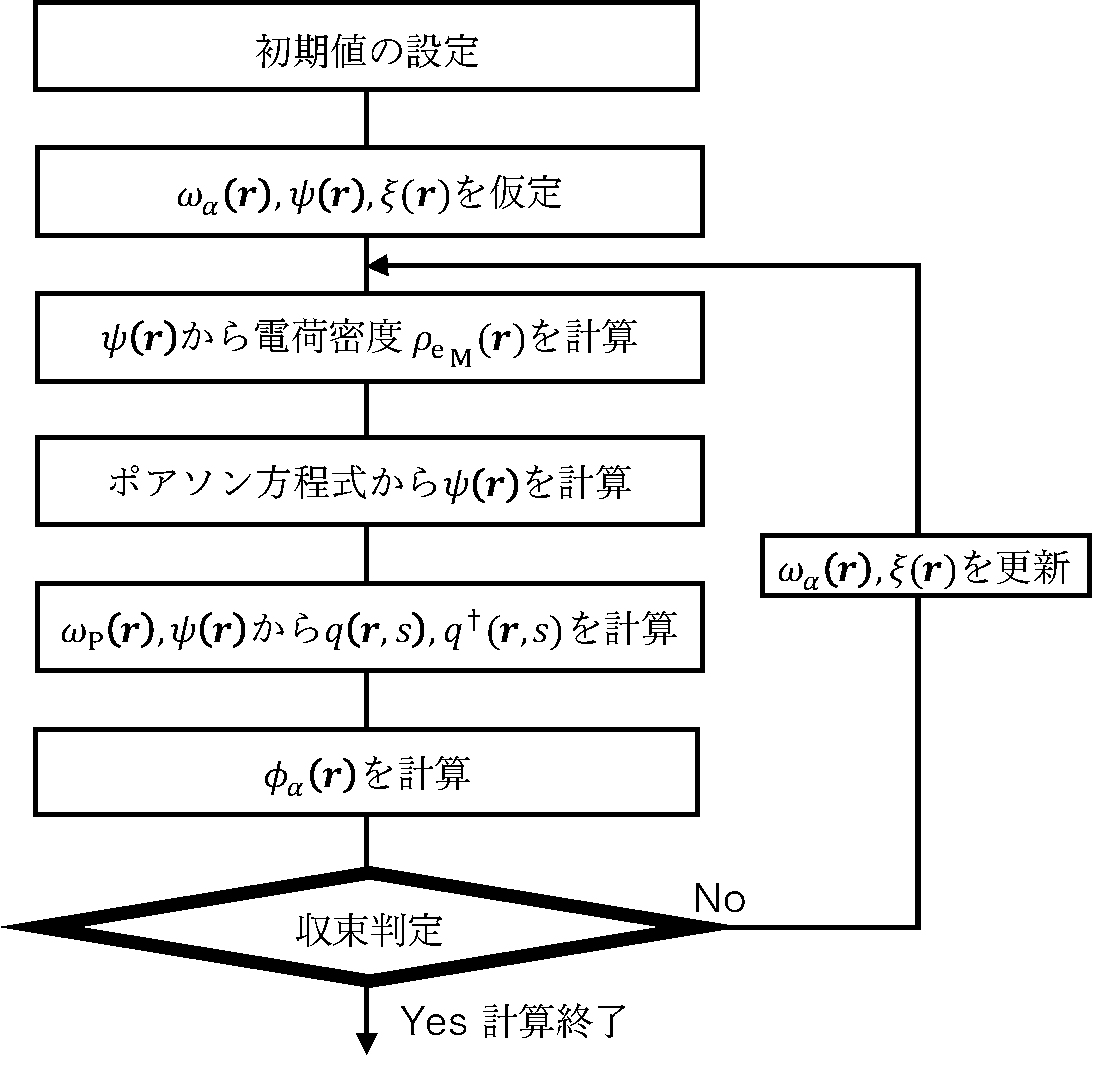
\includegraphics[keepaspectratio,scale=0.5]{Fig/Fig.2/SimulationMethod.pdf}
            \caption{自己無撞着場理論の計算フローチャート}
            \label{Fig.2-2-1}
\end{figure}
%
%
グラフト鎖の統計的重率の初期値は,端がコロイド表面にグラフトしていることから,コロイド表面近傍で$q(0,\bvec{r}_0)=1$とし,それ以外の場所で$q(0,\bvec{r})=0$とした.BispCにおける計算では,図$\ref{Fig.2-2-2}$に示したような微小厚み$\delta_{\rm{s}}$に1を与えた.ここで,$r_0$は無次元化したコロイド半径であり,$\delta_{\rm{s}}$も無次元化した厚みである.
%
\begin{figure}[H]
            \centering
            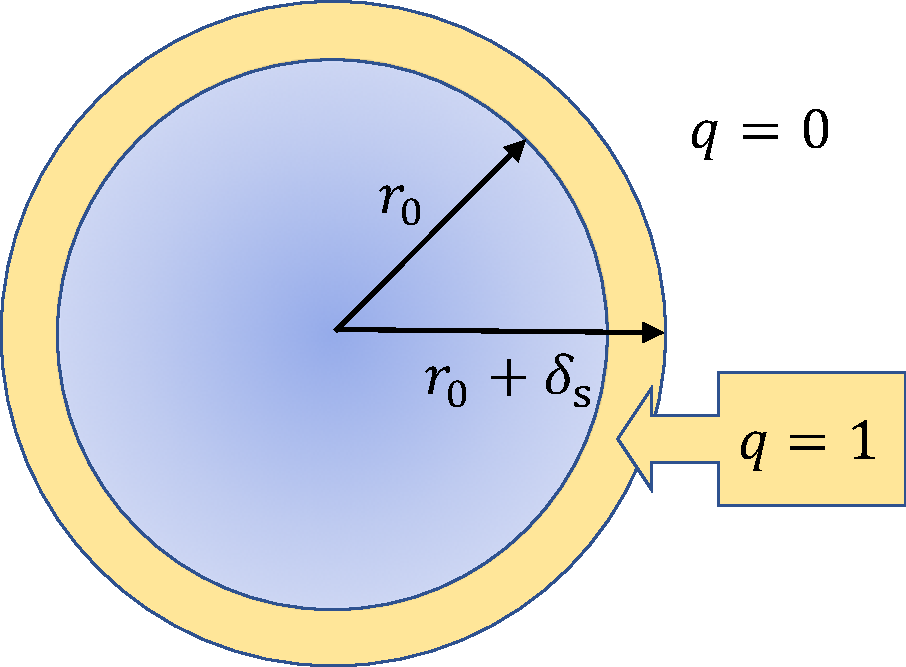
\includegraphics[keepaspectratio,scale=0.5]{Fig/Fig.3/inicial.pdf}
            \caption{グラフト鎖の初期条件における微小厚み$\delta_{\rm{s}}$}
            \label{Fig.2-2-2}
\end{figure}
%
自由鎖の統計的重率の初期値は,高分子鎖の末端は任意の位置に配位することができるため,任意の位置で$q^{\dag}(0,\bvec{r})=1$を与えた.また境界条件は,高分子ブラシがコロイド内部に配置できないようにコロイド表面で$q(s,\bvec{r}_{\rm{wall}})=0,q^{\dag}(s,\bvec{r}_{\rm{wall}})=0$とした.他の変数の初期値は0とした.
次にポテンシャル場$\omega_{\alpha}(\bvec r)$,$\psi(\bvec{r})$,$\xi(\bvec{r})$を$0$として仮定する.
仮定した$\psi(\bvec{r})$から電荷密度$\rho_{\rm{eM}}(\bvec{r})$を計算し,その電荷密度からポアソン方程式を用いて,電位$\psi(\bvec{r})$を計算する.
ポテンシャル場$\omega_{\alpha}(\bvec r), \psi(\bvec{r})$と配位の統計的重率の初期値$q(\bvec r, 0)$を用いて式 $ (\ref{eq2-1-1}) $に示す方程式を$s=0$から$s=1$まで解く.  $q^{\dag}(\bvec r, s)$についても同様に求める.
ここまでで,$q(\bvec r, s)$と$q^{\dag}(\bvec r, s)$が求められるため,式 $ (\ref{eq2-1-2}) $を用いて体積分率$\phi_{\alpha}(\bvec r)$を計算する.
計算された$\phi_{\alpha}(\bvec r)$と仮定した$\omega_{\alpha}(\bvec r)$から式 $ (\ref{eq2-1-11}) $から式 $ (\ref{eq2-1-13}) $に示す条件を満たしているか判定する.満たしている場合は仮定したポテンシャル場と計算された体積分率の値が矛盾なく成立していることになり,計算を終了する.満たしていない場合,ポテンシャル場と体積分率が矛盾していることになるため,仮定したポテンシャル場を$\omega_{\alpha} (\bvec r) = \omega_{\alpha} (\bvec r) + \delta \omega_{\alpha} (\bvec r)$を用いて更新し,再び仮定したポテンシャル場とし,同様に収束計算を行う.
%%%%%%%%%%%%%%%%%%%%%%%%%%%%%%%%%%%%%
\newpage
%%%%%%%%%%%%%%%%%%%%%%%%%%%%%%%%%%%%%
\subsection{Bispherical Coordinateの導入}
%%%%%%%%%%%%%%%%%%%%%%%%%%%%%%%%%%%%%
緒言でも述べたように,コロイド半径と高分子ブラシの回転慣性半径が同程度の場合を考えるため,コロイド表面の曲率を考慮することを考えた.そこで,本研究では,Bispherical Coordinate System(以降,BispC)という座標系を導入することとした.BispCは図\ref{Fig.2-3-1}のような座標系である.青破線と赤線の交点を格子点としており,本シミュレーションでは,格子点が存在しない二つの球面空間をコロイドと想定している.BispCは$a, \tau_{0}$,変数$\sigma, \tau$の刻み幅を指定することで座標系が決まる.直交座標との対応は,$\tau=\tau_0, -\tau_0$は左図のコロイド表面であり,$\tau=0$は$x$軸上を表す.$\sigma=0,  \pi$は$z$軸上かつ,それぞれコロイド間,その反対側の座標となる.
%
\begin{figure}[H]
		\centering
            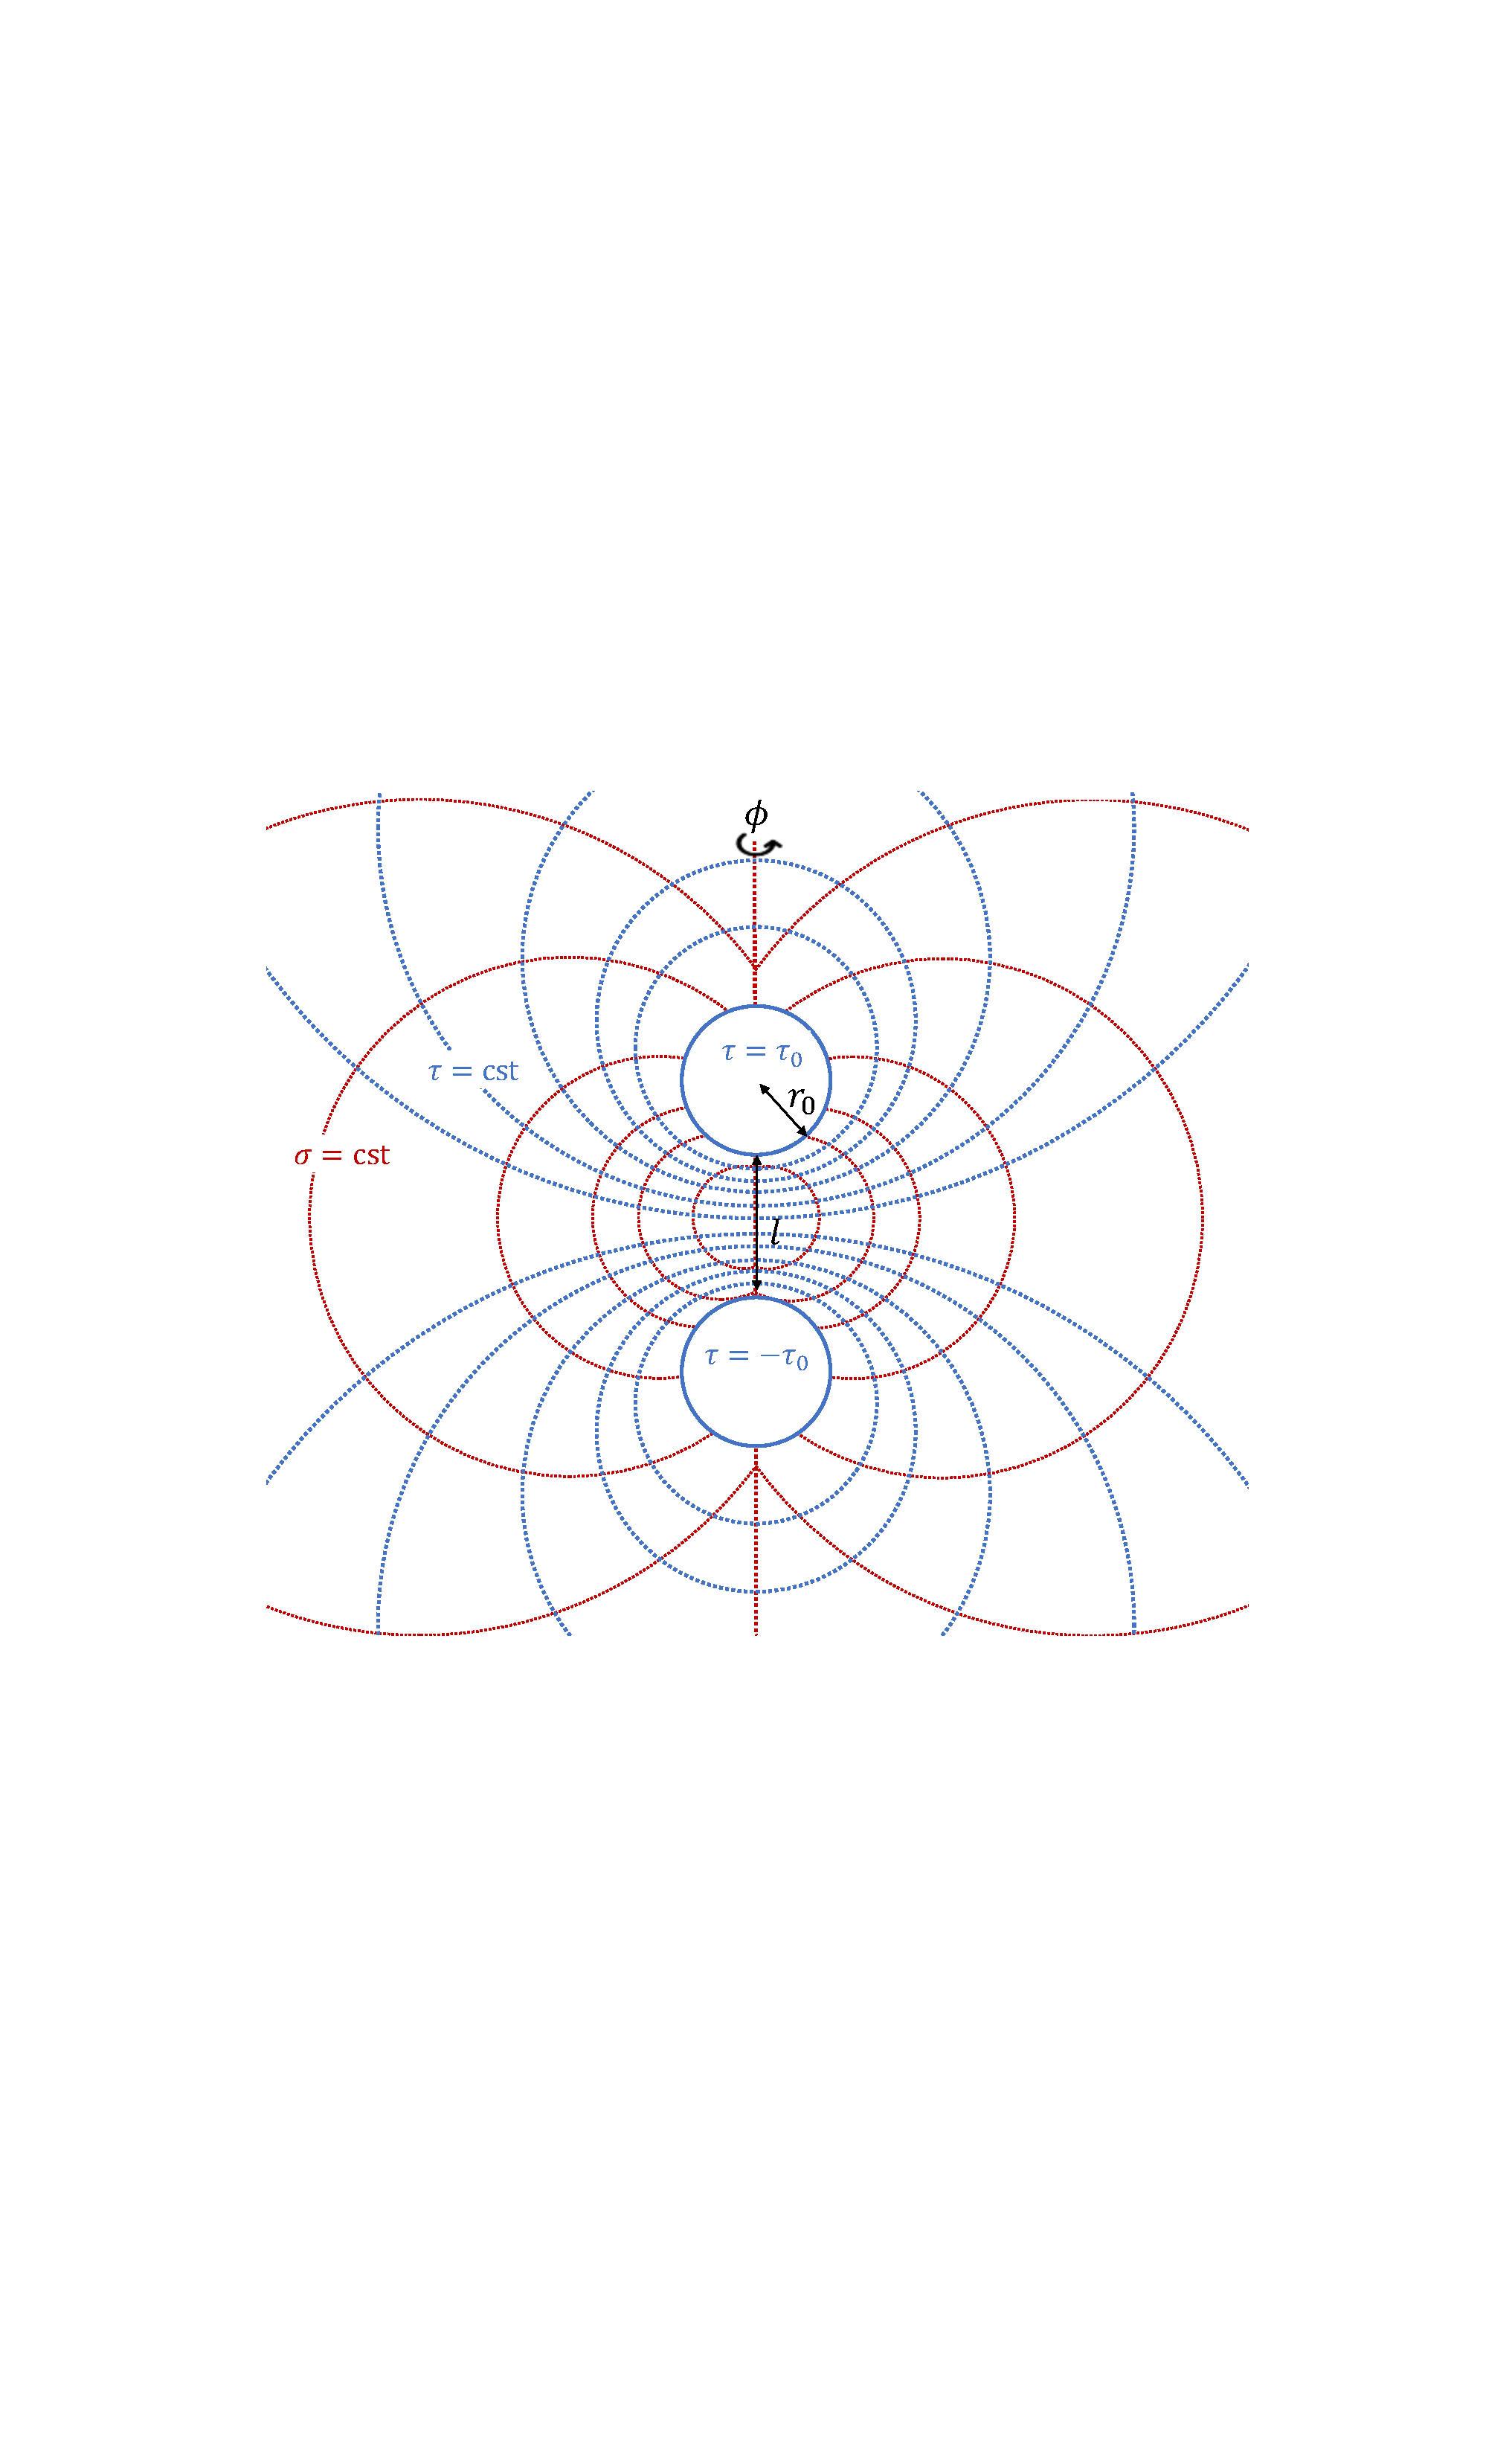
\includegraphics[keepaspectratio,scale=0.3]{Fig/Fig.4/BispC3.pdf}
            \hspace{10mm}
            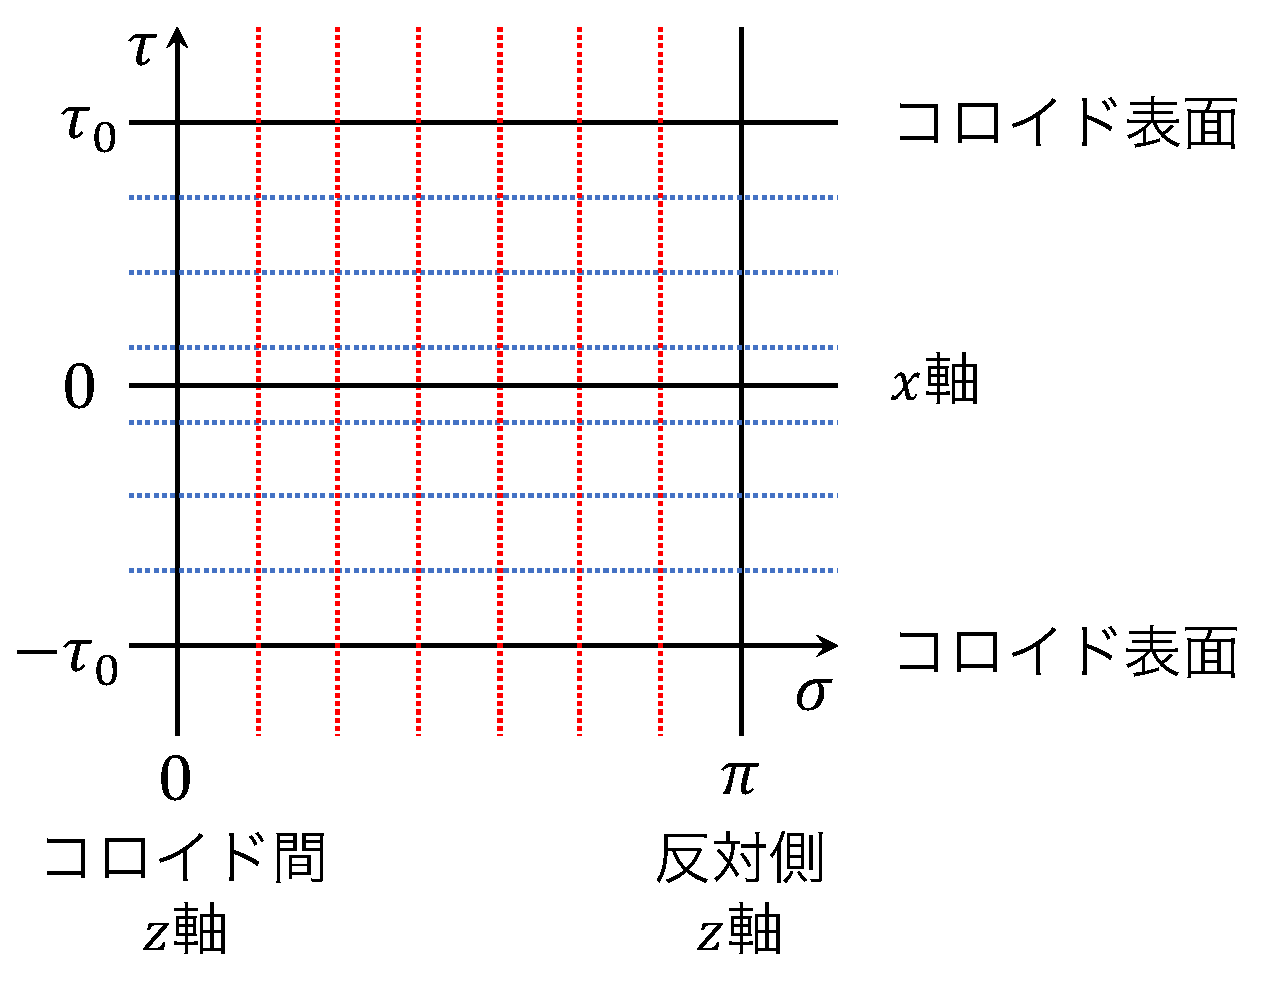
\includegraphics[keepaspectratio,scale=0.3]{Fig/Fig.4/BispC_Grid.pdf}
            \caption{BispC概略図}
\            \label{Fig.2-3-1}
\end{figure}
%
また,$a, \tau_{0}$はコロイド半径とコロイド間距離から式$(\ref{eq2-3-1})$, 式$(\ref{eq2-3-2})$計算される.
%
\begin{equation}
	\label{eq2-3-1}
	\tau_{0}={\rm{ln}}\Bigl[\frac{l}{2r_0}+1+\sqrt{\Bigl(\frac{l}{2r_{0}}\Bigr)^{2}+\frac{l}{r_{0}}}\,\Bigr]
\end{equation}
%
%
\begin{equation}
	\label{eq2-3-2}
	a=r_{0}\rm{sinh}\tau_{0}
	\end{equation}
%
計算範囲は対称性を利用して,$-\tau_{0}<\tau<\tau_{0}$, $0<\sigma<\pi$とし,$\phi$は軸対称として計算した.媒介変数$\sigma,  \tau$から直交座標系への変換は,式$(\ref{eq2-3-3})$によって行われる.
%
\vspace{-10mm}

\begin{align}
\label{eq2-3-3}
		x = a \frac{\rm{sin}\sigma}{\rm{cosh}\tau-\rm{cos}\sigma} \rm{cos}\phi,\,\,\,\,\,\,\,\,\,\,\,\,
	&    y = a \frac{\rm{sin}\sigma}{\rm{cosh}\tau-\rm{cos}\sigma} \rm{sin}\phi,
	&    z= a \frac{\rm{sinh}\tau}{\rm{cosh}\tau-\rm{cos}\sigma}
\end{align}
%
\vspace{1mm}
式$(\ref{eq2-3-4}),(\ref{eq2-3-5})$はそれぞれ,図\ref{Fig.2-3-1}の赤破線,  青破線を表している.
%
\begin{equation}
	\label{eq2-3-4}
	z^{2}+(\sqrt{x^{2}+y^{2}}-a{\rm{coth}}\sigma)^{2}=\frac{a^{2}}{{\rm{sin}}^{2}\sigma}
\end{equation}
%
%
\begin{equation}
	\label{eq2-3-5}
	(x^{2}+y^{2})+(z-a{\rm{coth}}\tau)^{2}=\frac{a^{2}}{{\rm{sinh}}^{2}\tau}
\end{equation}
%
\vspace{1mm}
式$(\ref{eq2-3-6})$はBispCにおけるラプラシアンの式であり,式$(\ref{eq2-3-6})$はBispCにおけるヤコビアンの式である.
%
\begin{equation}
	\label{eq2-3-6}
	\begin{split}
	\nabla^{2}\Phi = \frac{1}{\bvec{J}}&
	\Bigl[\frac{\partial}{\partial \sigma}\Bigl(\frac{{\rm{sin}}\sigma}{{\rm{cosh}}\tau-{\rm{cos}}\sigma} \frac{\partial\Phi}{\partial\sigma} \Bigr)
	+ \frac{\partial}{\partial \tau}\Bigl(\frac{{\rm{sin}}\sigma}{{\rm{cosh}}\tau-{\rm{cos}}\sigma} \frac{\partial\Phi}{\partial\tau} \Bigr) 
	+ \frac{\partial^{2}}{\partial\phi^{2}}\frac{\Phi}{{\rm{sin}}\sigma({\rm{cosh}}\tau-{\rm{cos}}\sigma)}\Bigr]
	\end{split}
\end{equation}
%
%
\begin{equation}
	\label{eq2-3-7}
		\bvec{J} = \frac{a^{2}{\rm{sin}}\sigma}{({\rm{cosh}}\tau-{\rm{cos}}\sigma)^{3}}
\end{equation}
%
%%%%%%%%%%%%%%%%%%%%%%%%%%%%%%%%%%%%%
\newpage
%%%%%%%%%%%%%%%%%%%%%%%%%%%%%%%%%%%%%
%%%%%%%%%%%%%%%%%%%%%%%%%%%%%%%%%%%%%
\section{シミュレーション結果と考察}
%%%%%%%%%%%%%%%%%%%%%%%%%%%%%%%%%%%%%
%%%%%%%%%%%%%%%%%%%%%%%%%%%%%%%%%%%%%
\subsection{1次元系(平行平板間のグラフト鎖)での計算結果}
コロイド半径が高分子ブラシの回転慣性半径よりも十分に大きいとし,コロイド表面を平坦としてシミュレーションを行った.つまり,ここでのシミュレーションは1次元で行っている.
%%%%%%%%%%%%%%%%%%%%%%%%%%%%%%%%%%%%%
\vspace{-3mm}
%%%%%%%%%%%%%%%%%%%%%%%%%%%%%%%%%%%%%
\subsubsection{電離度について}
%%%%%%%%%%%%%%%%%%%%%%%%%%%%%%%%%%%%%
高分子ブラシが電離している割合のことを電離度と呼ぶこととする.また,計算を簡易化するため,高分子ブラシは一様に電離度$p$で電離しているモデル(Smear Model)を用いた. .
%
\begin{figure}[H]
		\centering
            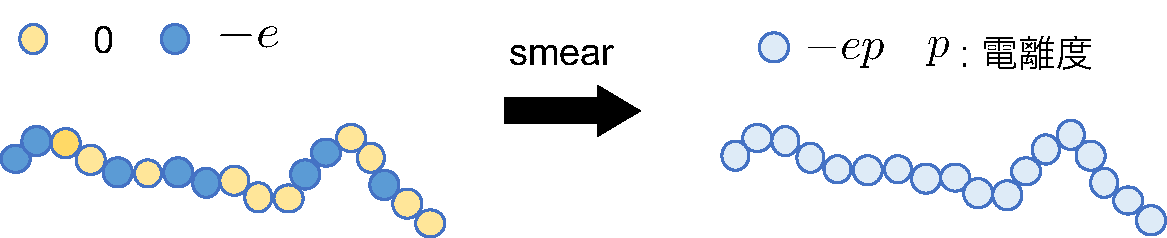
\includegraphics[keepaspectratio,scale=0.5]{Fig/Fig.5/smear.pdf}
            \caption{電離模式図1}
\            \label{Fig.3-1-1}
\end{figure}
%
 今回用いたsmear modelに対して,anneal modelを紹介する.本研究では,計算簡易化のためsmear modelを用いたが,電離度が小さい場合はanneal modelを用いる.anneal modelでは,高分子鎖上の位置によって持つ電荷に分布が存在し,それは電位の分布に依存する.高分子鎖の持つ電荷は式$(\ref{eq3-1-1})$で表され,ポテンシャル場は式$(\ref{eq3-1-2})$となる.
%
\begin{figure}[H]
		\centering
            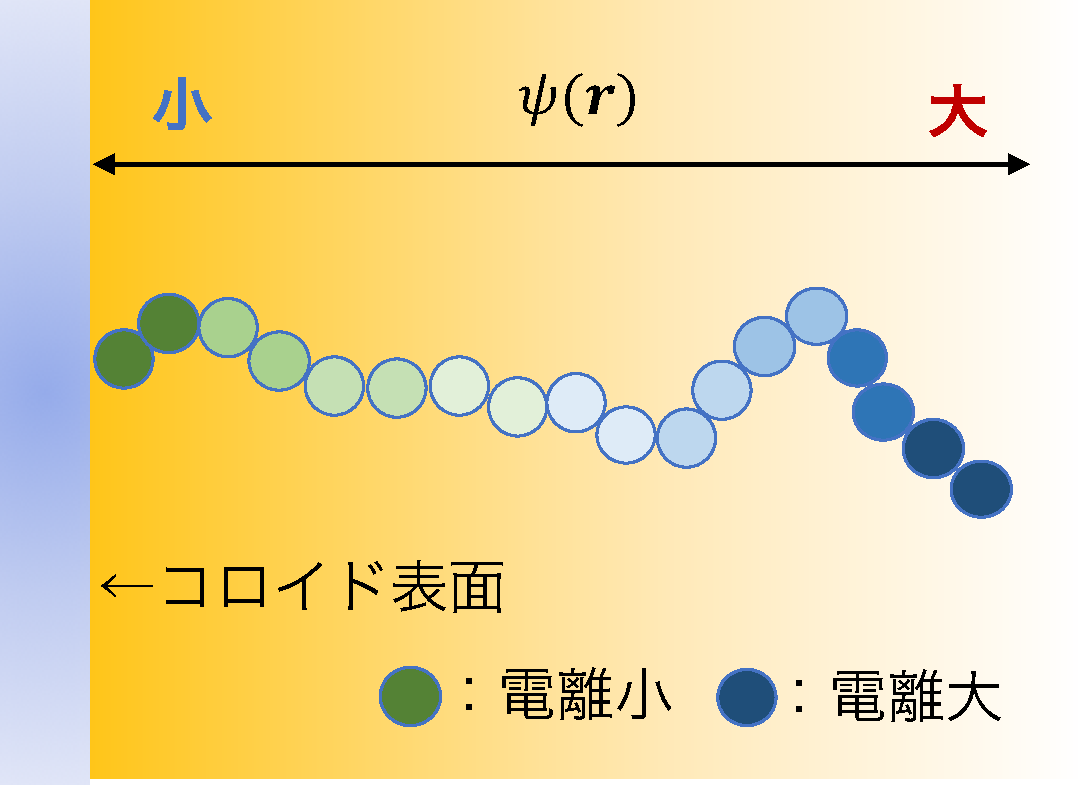
\includegraphics[keepaspectratio,scale=0.4]{Fig/Fig.6/anneal.pdf}
            \caption{電離模式図2}
\            \label{Fig.3-1-2}
\end{figure}
%
%
\begin{equation}
	\label{eq3-1-1}
	\rho_{\rm{eP}}(\bvec{r})=-ep\phi_{\rm{P}}(\bvec{r})\frac{1}{p+(1-p)e^{-e\psi(\bvec{r})}}
	\end{equation}
%
%
\begin{equation}
	\label{eq3-1-2}
	\Omega(\bvec{r})=\omega_{\rm{P}}(\bvec{r})-{\rm{ln}}\Bigl[1-p+p{\rm{e}}^{ep\psi(\bvec{r})}\Bigr]
	\end{equation}
%
\vspace{-10mm}
%
%%%%%%%%%%%%%%%%%%%%%%%%%%%%%%%%%%%%%
\subsubsection{グラフト密度について}
高分子ブラシの回転慣性半径は,隣り合う高分子鎖との相互作用でその大きさを変える.つまり,隣り合う高分子鎖のグラフト点間距離が,高分子ブラシの広がりの大きさ($R_g$)よりも十分遠い場合,フラフと高分子のセグメント密度分布は,マッシュルーム型と呼ばれる壁面方向に広がった濃度分布を示すのに対し,グラフト点間距離が$R_g$よりも小さくなると,高分子鎖間の排除体積効果により,壁面に対し垂直な方向へ延びる. ここでは,隣り合う高分子ブラシが相互作用をするグラフト密度範囲を調べる.図$\ref{Fig.3-1-1-2}$で,グラフト密度と高分子ブラシの回転慣性半径の関係を示した.高分子ブラシの回転慣性半径が変化しなくなるグラフト密度で,高分子鎖は隣の高分子鎖からの影響を受けていないとした.今回の条件では,$\sigma_{\rm{P}}a^2=7.0\times10^{-4}$付近で,高分子ブラシの回転慣性半径が一定(マッシュルーム型の濃度分布領域)となっていることがわかる.
\begin{figure}[H]
		\centering
            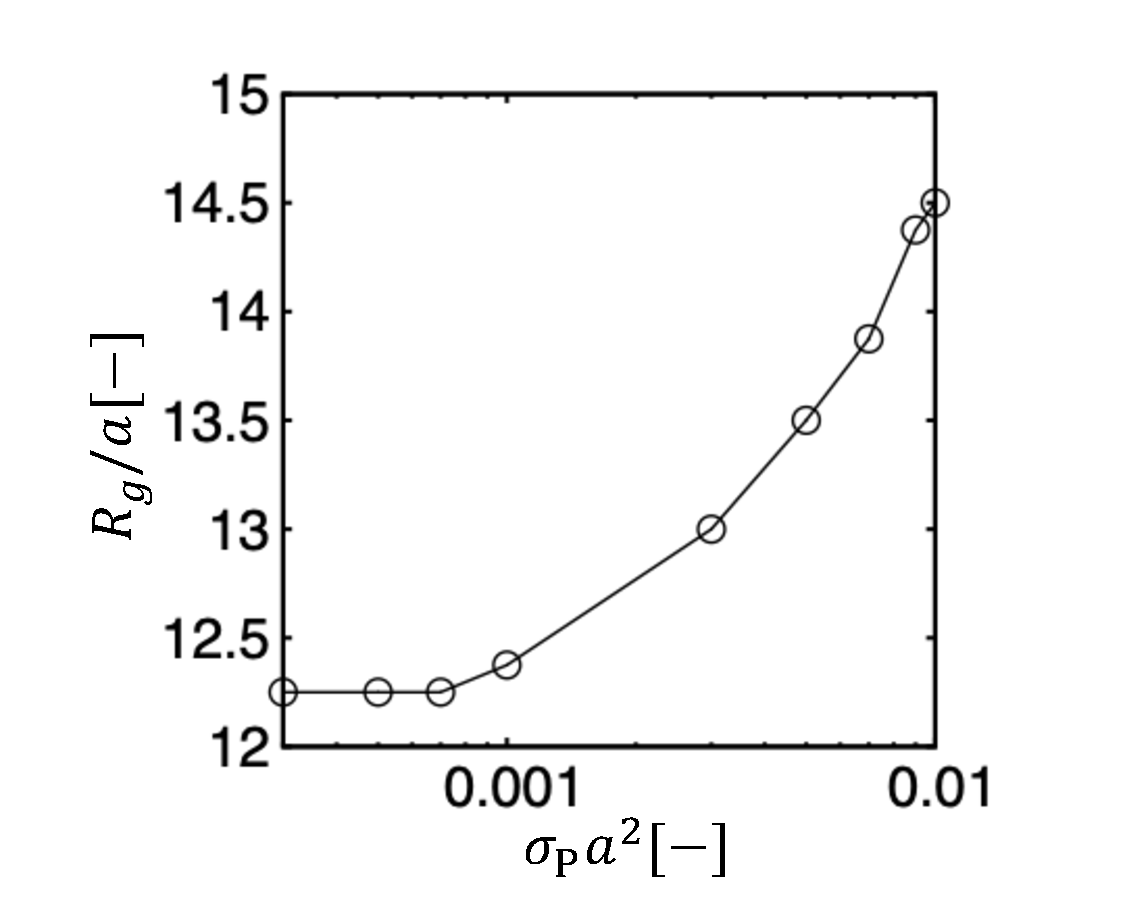
\includegraphics[keepaspectratio,scale=0.5]{Fig/Fig.7/sigma_Rg.pdf}
            \caption{グラフト密度と高分子ブラシの回転慣性半径の関係}
\            \label{Fig.3-1-1-2}
\end{figure}
これらの結果から,図$\ref{Fig.3-1-1-3}$で高分子ブラシをまっすぐに伸ばした時の長さ(鎖長$Na$),
,回転慣性半径,間隔を模式的に示した.今回,高分子ブラシのセグメント数$N=100$としていることから,高分子ブラシの鎖長は$100a$であり,長さの基準として図$\ref{Fig.3-1-1-3}$のそれぞれ上方に示した.$\sigma_{\rm{P}}a^2=1.0\times10^{-2}$では,グラフト点間距離が$10.0a$であり,$19.0a$だけ高分子鎖の分布範囲が重なっている.
\begin{figure}[H]
		\centering
            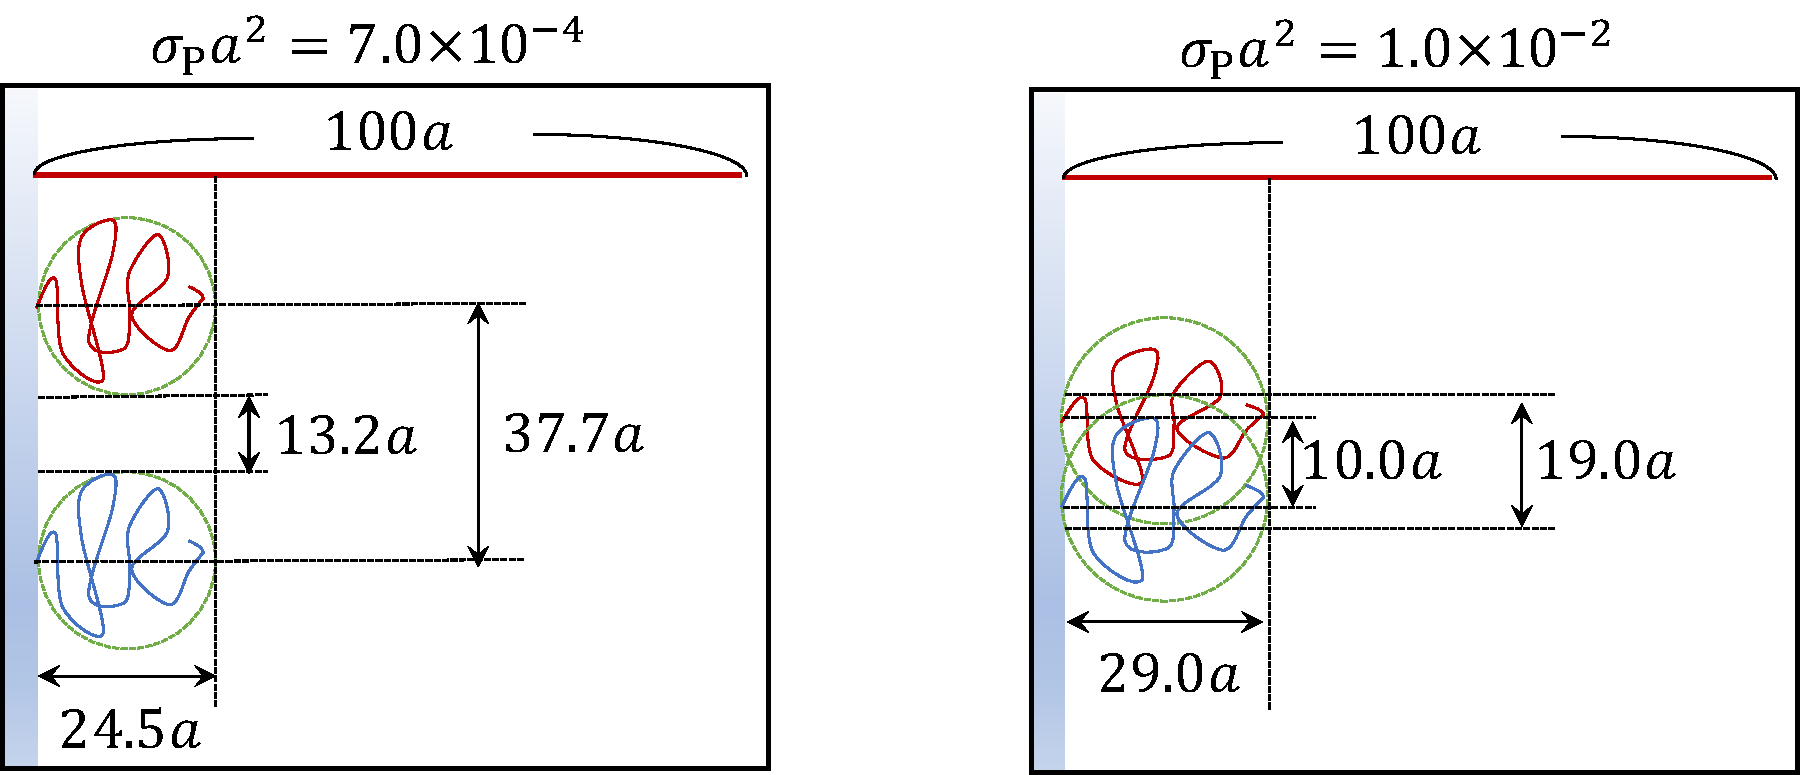
\includegraphics[keepaspectratio,scale=0.4]{Fig/FIg.8/graft_Rg.pdf}
            \caption{高分子ブラシ系での幾つかの特徴的な長さ間の関係を表す模式図}
\            \label{Fig.3-1-1-3}
\end{figure}

%%%%%%%%%%%%%%%%%%%%%%%%%%%%%%%%%%%%%
\subsubsection{電離度に対する体積分率・電荷密度分布の変化}
%%%%%%%%%%%%%%%%%%%%%%%%%%%%%%%%%%%%%
ここでは,セグメント数$N=100$,グラフト密度$\sigma_{\rm{P}}a^2=0.01$とし,相互作用パラメータ$\chi$は,溶媒が良溶媒であることを想定して$\chi=0.10$とした.システムサイズは電荷密度がコロイド表面から離れた場所で一定とみなせる距離とし,$L_x/a=80$とした.計算で用いたパラメータの一覧を次の表\ref{table2-7-2}に示す.
%%%%%%%%%%%%%%%%%%%%%%%%%%%%%%%%%%%%%
\begin{table}[htb]
    \caption{計算に用いたパラメータ}
    \vspace{-1.50 zh}
    \begin{center}
        \begin{tabular}{ll}\hline
            x方向のシステムサイズ & $L_x/a = 80 $\\ \\
            グラフト密度 & $\sigma_{\mathrm p}a^{2} = 0.01$\\ \\
            高分子鎖のセグメント数 & $N = 100$\\ \\
            高分子ブラシ,\,溶媒間相互作用パラメータ & $\chi = 0.10$\\ \hline
        \end{tabular}
    \end{center}
        \label{table2-7-2}
\end{table}\\
%%%%%%%%%%%%%%%%%%%%%%%%%%%%%%%%%%%%%

%%%%%%%%%%%%%%%%%%%%%%%%%%%%%%%%%%%%%
 計算結果を図$\ref{Fig3-1-2}$に示す.図$\ref{Fig3-1-2}(\rm{a})(\rm{b})$はそれぞれ,高分子ブラシの体積分率と電荷密度の分布を表している.$x/a$は壁面からの距離を表す.(a)のグラフから,電離度$p$が増加するに従って,高分子ブラシはその分布範囲を広げていることがわかる.これは,電離度が増加することで,溶媒中に含まれる正電荷が増加し,正電荷は自らのエントロピーを増大させようとする.それに対して,正電荷は負電荷を持つ高分子ブラシから離れられない.この二つの効果から,図$\ref{Fig3-1-3}$のように高分子ブラシに浸透圧が働き,高分子ブラシはその分布範囲を広げる.その傾向が図$\ref{Fig3-1-2}(\rm{a})$によく表れている.電荷密度に関しては,正電荷は高分子ブラシの近くに多く存在することとなり,遠方で0となる.コロイド表面近傍では高分子ブラシが少ないことから,コロイド表面近傍で電荷密度は正となり,高分子ブラシが多く存在するところで負,そして,高分子ブラシが少なくなると正となる.また,電荷密度の正側の極値をもつ位置は,高分子ブラシの広がりと共にコロイド表面から離れる.これらの傾向は,図$\ref{Fig3-1-2}(\rm{b})$のグラフでも見られる.
\newpage
%%%%%%%%%%%%%%%%%%%%%%%%%%%%%%%%%%%%%
\begin{figure}[h]
\centering
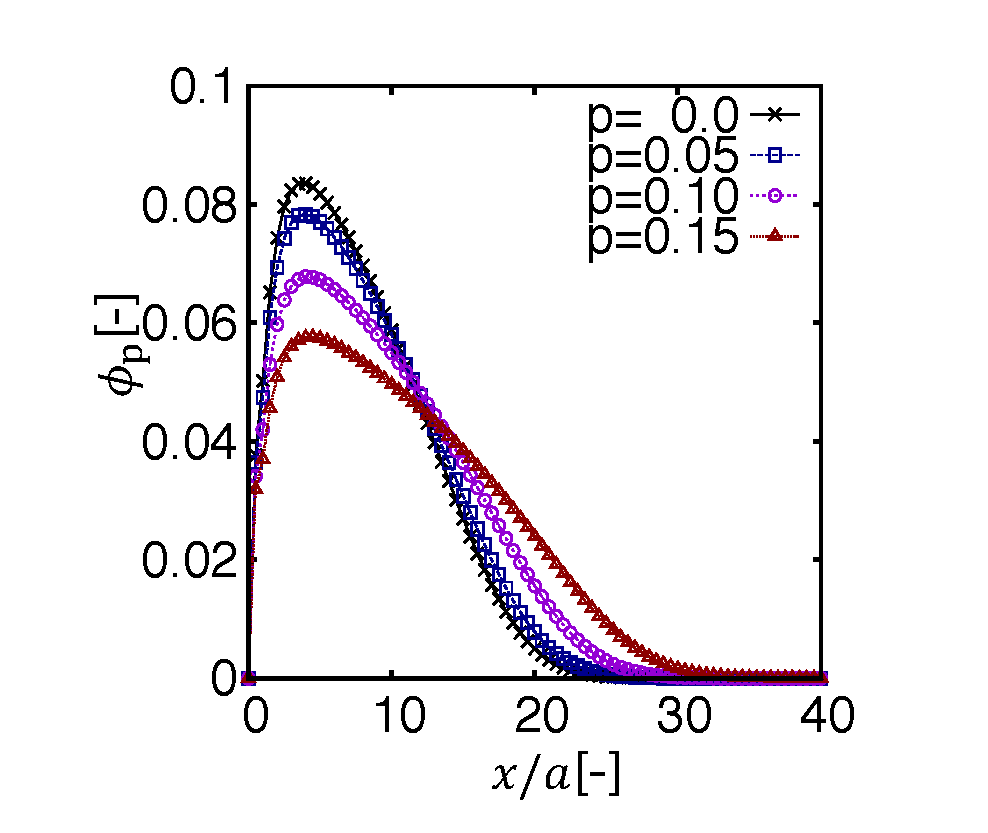
\includegraphics[width=65.5mm]{Fig/Fig.9/phip.pdf}
\put(-180,130){(a)}
\hspace{2zh}
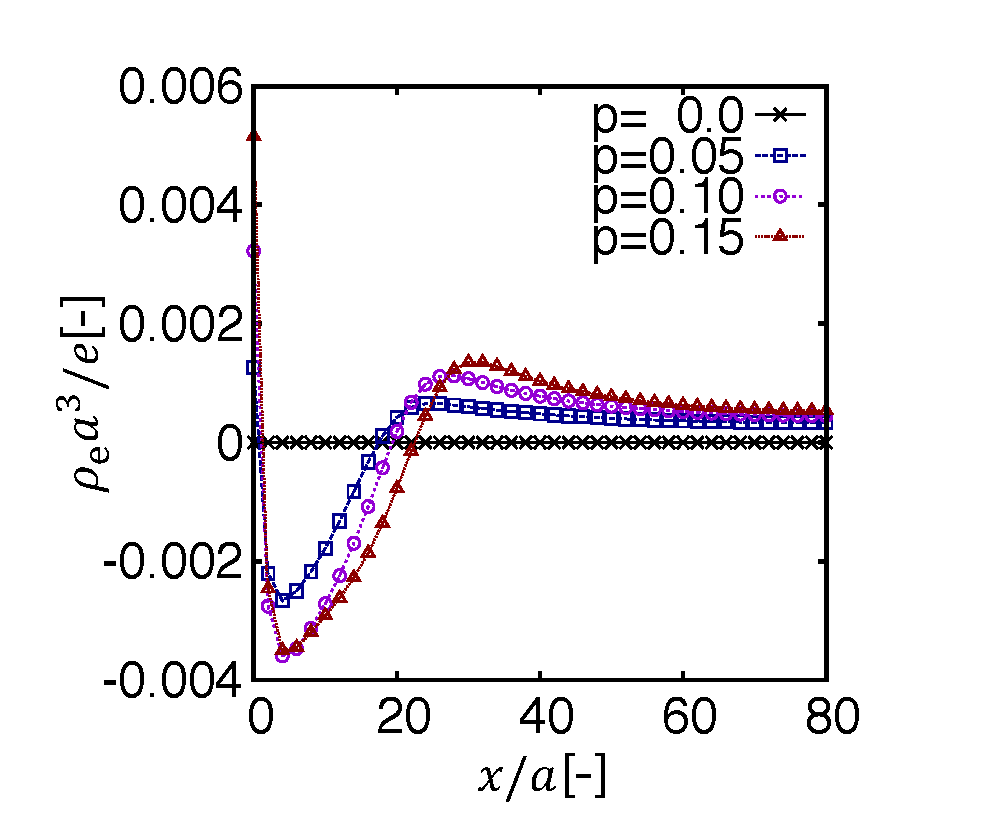
\includegraphics[width=65.5mm]{Fig/Fig.9/rho.pdf}
\put(-185,130){(b)}
\caption{(a)高分子ブラシの体積分率分布 (b)電荷密度分布}
\label{Fig3-1-2}
\end{figure}
%%%%%%%%%%%%%%%%%%%%%%%%%%%%%%%%%%%%%
%%%%%%%%%%%%%%%%%%%%%%%%%%%%%%%%%%%%%
\begin{figure}[h]
\centering
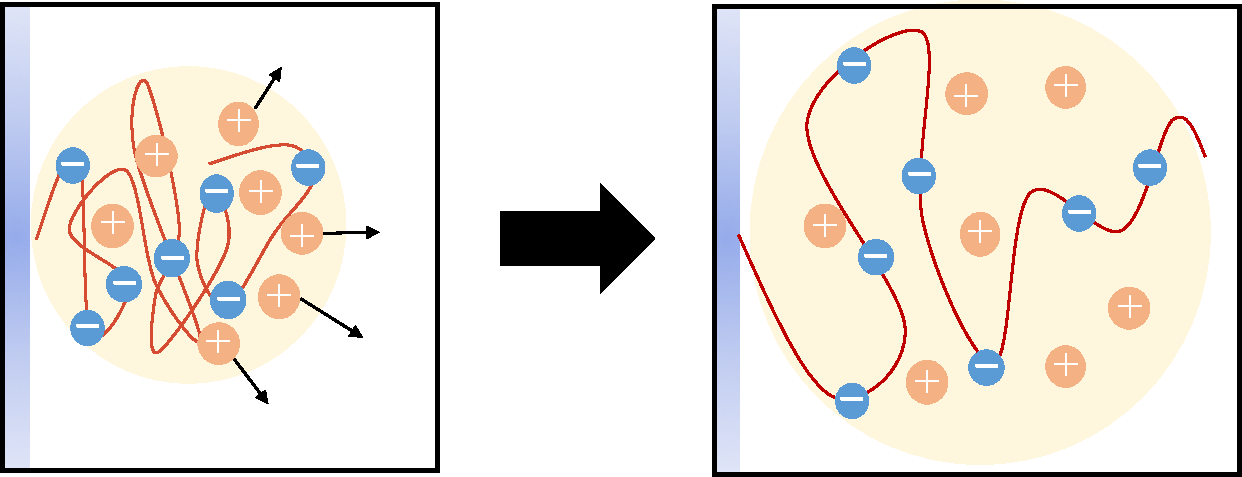
\includegraphics[width=120mm]{Fig/Fig.10/shintoatu.pdf}
\caption{電離したイオンよる浸透圧の模式図}
\label{Fig3-1-3}
\end{figure}
%%%%%%%%%%%%%%%%%%%%%%%%%%%%%%%%%%%%%
\newpage
%%%%%%%%%%%%%%%%%%%%%%%%%%%%%%%%%%%%%
%%%%%%%%%%%%%%%%%%%%%%%%%%%%%%%%%%%%%
\subsection{Bispherical Coordinate Systemを用いた計算結果}
%%%%%%%%%%%%%%%%%%%%%%%%%%%%%%%%%%%%%
%%%%%%%%%%%%%%%%%%%%%%%%%%%%%%%%%%%%%
\subsubsection{壁面の曲率が高分子ブラシの平衡構造に与える影響}
%%%%%%%%%%%%%%%%%%%%%%%%%%%%%%%%%%%%%
コロイド半径が高分子ブラシの回転慣性半径よりも十分に大きい場合,コロイド表面を平坦として計算できたが,本研究では,コロイド半径が高分子ブラシの回転慣性半径と同程度の場合を考えるため,あるいは,コロイド間相互作用をより適切にシミュレーションすることが可能となるように,BispCを導入した.ここでは,BispCでの計算結果と壁面が平坦な場合での計算結果を比較することで,曲率がシミュレーション結果に与える影響を調べ,同時にBispCでの計算結果の妥当性を示す.また,壁面が平坦な場合の計算結果は無次元化したコロイド半径$r_0=\infty$に対応している.図$\ref{Fig3-2-1}(\rm{a})$では,無次元化したコロイド半径$r_0$を変化させた際の高分子ブラシの体積分率の分布となっている.
 図$\ref{Fig3-2-1}$(a)からわかるように,曲率が大きいほど,つまりコロイド半径が小さいほど,高分子セグメント体積分率$\phi_{\rm P}$の値が小さくなっている.また,曲率が大きいほど,体積分率の最大値の位置がコロイド表面近傍に接近している.これら二つの傾向は,曲率の増加によって,高分子ブラシの半径方向以外への広がりが増加するからだと考えられる.コロイド表面を平坦とした場合,対称性から半径方向の広がりのみを計算すればよい.曲率が増加すると図$\ref{Fig3-2-1}(\rm{b})$から分かるように,半径方向にコロイド表面から離れるにつれて,高分子ブラシ間に余計に空間が生まれる.これが高分子ブラシの半径方向以外への広がりの原因である.
%%%%%%%%%%%%%%%%%%%%%%%%%%%%%%%%%%%%%
\begin{figure}[h]
\centering
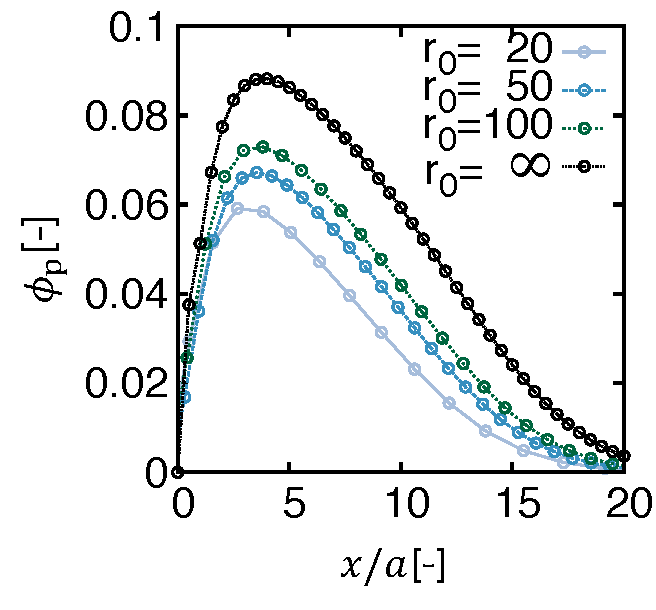
\includegraphics[width=60mm]{Fig/Fig.11/curve.pdf}
 \put(-190,130){(a)}
\hspace{6zh}
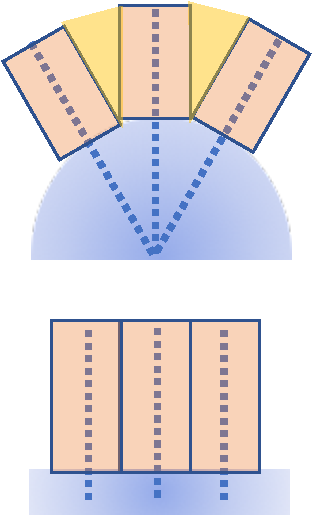
\includegraphics[width=35mm]{Fig/Fig.11/space_curve.pdf}
 \put(-150,130){(b)}
\caption{(a)高分子ブラシの体積分率の分布,(b)曲率によって生じる空間の模式図}
\label{Fig3-2-1}
\end{figure}
%%%%%%%%%%%%%%%%%%%%%%%%%%%%%%%%%%%%%
%%%%%%%%%%%%%%%%%%%%%%%%%%%%%%%%%%%%%
\begin{table}[htb]
    \caption{計算に用いたパラメータ}
    \vspace{-1.5 zh}
    \begin{center}
        \begin{tabular}{ll}\hline
            グラフト密度 & $\sigma_{\mathrm p}a^{2} = 0.01$\\ \\
            高分子鎖のセグメント数 & $N = 100$\\ \\
            高分子ブラシ,\,溶媒間相互作用パラメータ & $\chi = 0.10$\\ \hline
        \end{tabular}
    \end{center}
        \label{table3-2-1}
\end{table}
%%%%%%%%%%%%%%%%%%%%%%%%%%%%%%%%%%%%%
%%%%%%%%%%%%%%%%%%%%%%%%%%%%%%%%%%%%%
\subsubsection{2つのコロイド間距離がグラフト高分子の平衡構造へ与える影響}
%%%%%%%%%%%%%%%%%%%%%%%%%%%%%%%%%%%%%
コロイド間相互作用を考えるため,無次元化したコロイド間距離$\ell=L/a=20と30$の場合についてシミュレーションを行った.ここでは,グラフト密度$\sigma_{\rm{P}}a^2=0.01$,セグメント数$N=100$,高分子,溶媒間の相互作用パラメータ$\chi=0.10$,電離度$p=0.10$とし,1価のイオンを$ N_{\rm{a}}a^3C=0.01$を加えることにした.
\begin{table}[htb]
    \caption{計算に用いたパラメータ}
    \vspace{-1.5 zh}
    \begin{center}
        \begin{tabular}{ll}\hline
            グラフト密度 & $\sigma_{\mathrm p}a^{2} = 0.01$\\ \\
            高分子鎖のセグメント数 & $N = 100$\\ \\
            高分子ブラシ,\,溶媒間相互作用パラメータ & $\chi = 0.10$\\ \\
            1価イオンの濃度 & $N_{\rm{A}}a^3C=0.01$\\ \hline
        \end{tabular}
    \end{center}
        \label{table3-2-1}
\end{table}

シミュレーション結果は,図$\ref{Fig3-3-1}$となった.図$\ref{Fig3-3-1}$(a)は高分子ブラシの体積分率を表しており,$\ell=20$では$\ell=30$と比較して,コロイド間で両コロイドの高分子ブラシが互いの領域にかなり入り込んでいることがわかる.電荷密度に関しても,コロイド間の中心あたりで$\ell=20$の場合に負であるのに対し,$\ell=30$の場合に電荷密度の値が一旦0まで上昇している.\\
%
\begin{figure}[h]
\centering
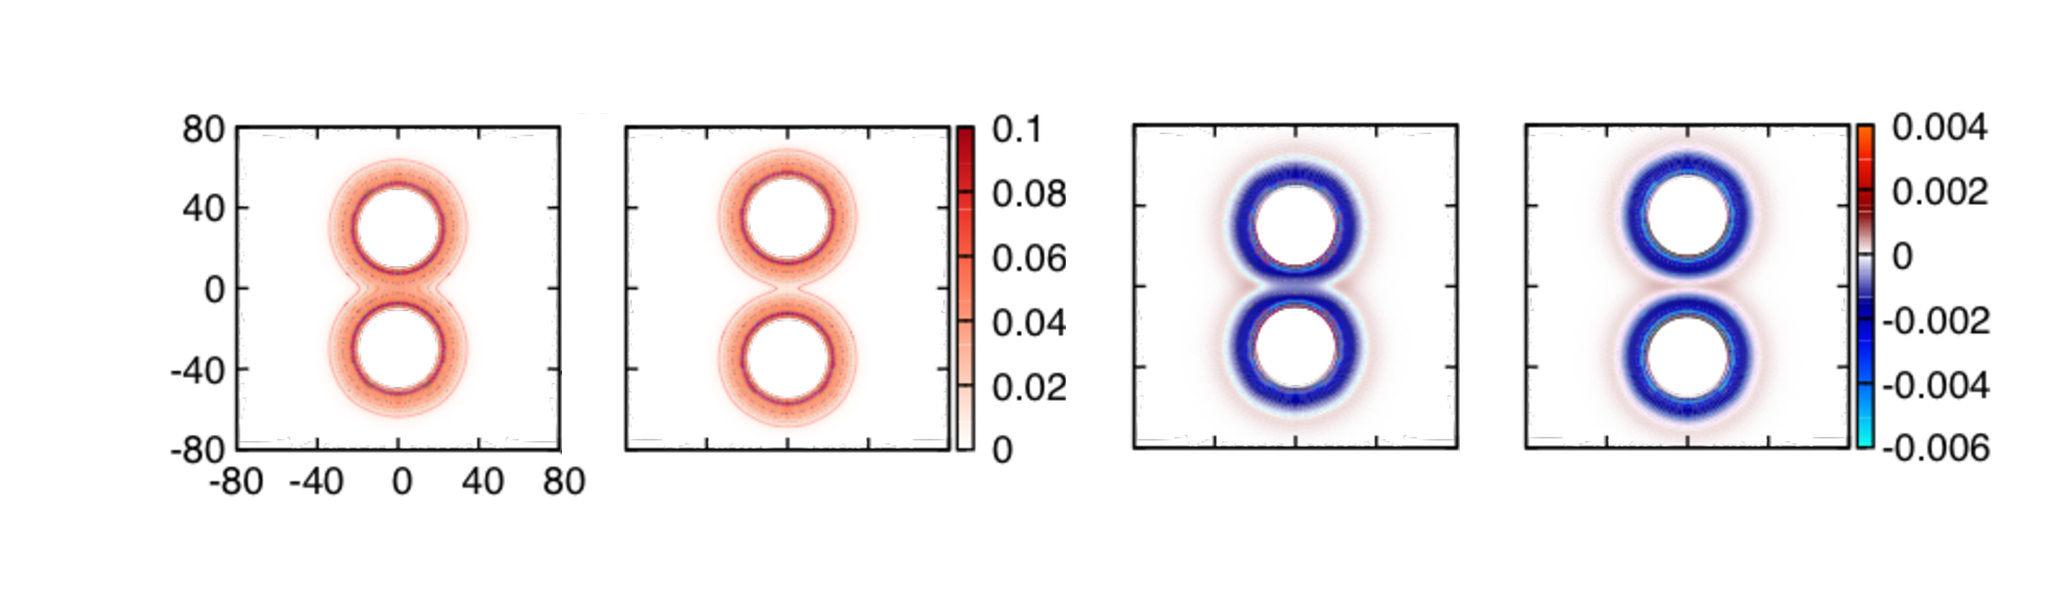
\includegraphics[width=160mm]{Fig/Fig.12/2colloid_VP_CD.pdf}
 \put(-435,80){(a-1)} 
 \put(-338,80){(a-2)}
 \put(-213,80){(b-1)}
 \put(-117,80){(b-2)}
\caption{(a-1)$\ell=20$での体積分率分布,(a-2)$\ell=30$での体積分率分布\\
\,\,\,\,\,\,\ \ \ \ \ (b-1)$\ell=20$での電荷密度分布,(b-2)$\ell=30$での電荷密度分布}
\label{Fig3-3-1}
\end{figure}
%

 コロイド間での高分子ブラシの体積分率と電荷密度の分布を詳しく見た結果を図$\ref{Fig3-3-2}$に示す.また,曲率がある場合とない場合を比較するため,同図にコロイド表面を平坦とした場合の計算結果も示す.体積分率に関しては,3.2.1での結果と同様の傾向が見られ,コロイド表面が平坦とした場合と比較して,体積分率の値は小さく,体積分率の最大値位置はコロイド表面近傍に接近している.また,$\ell=20$ではコロイド間の中心付近で体積分率の値がほぼ一定となっている.これは,両コロイドの高分子ブラシが互いの領域に十分に侵入していることを表している.次に電荷密度に関しては,コロイド表面が平坦とした場合と比較して,電荷密度の値が小さくなっていることがわかる.これは,正電荷は3-1-2で説明した挙動を示そうとするが,コロイド間では高分子ブラシが自らの分布範囲を広げることが困難である.結果,正電荷はより高分子ブラシの分布範囲を広げることが容易である場所へ分布し,コロイド間では電荷密度の値が小さくなると考えられる.この考察が正しいかは,コロイド間以外の箇所をより詳しく解析する必要があるが,それは今後の課題とする.

%
\begin{figure}[h]
\centering

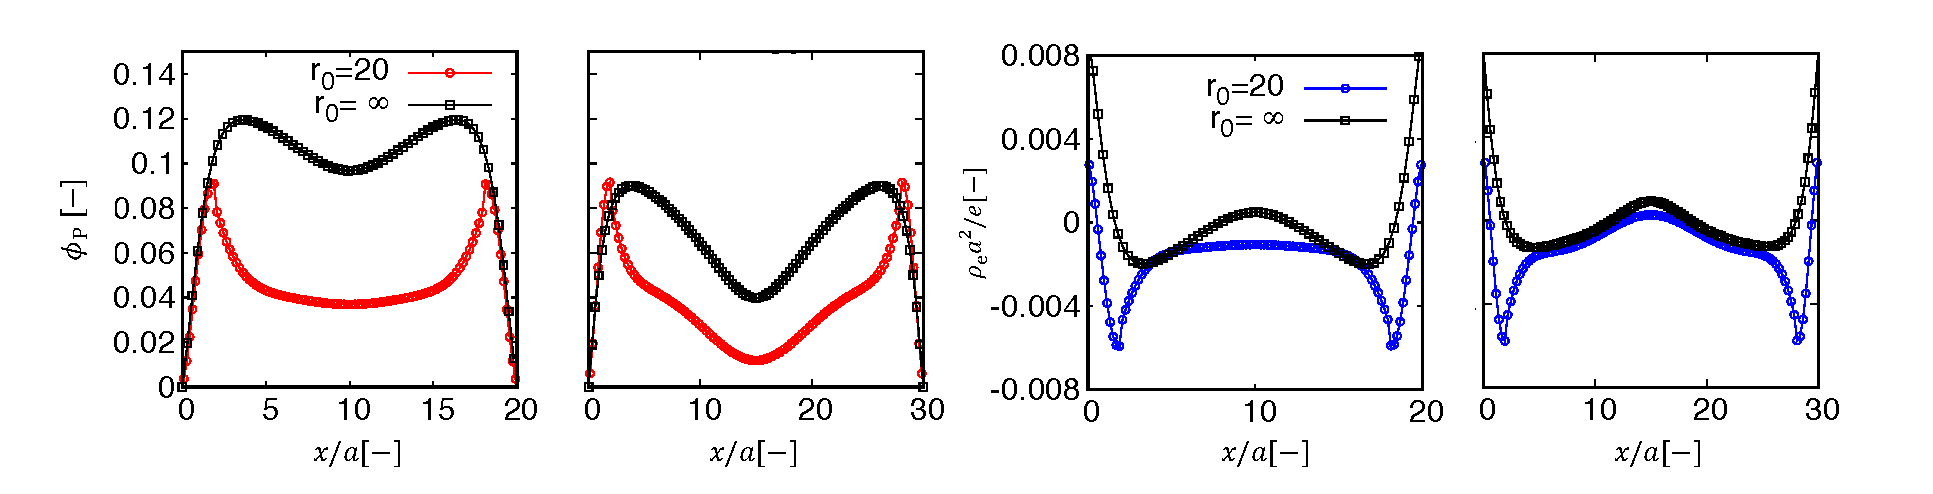
\includegraphics[width=155mm]{Fig/Fig.13/2colloid_1D.pdf}
 \put(-400,105){(a-1)} 
 \put(-310,105){(a-2)}
 \put(-195,105){(b-1)}
 \put(-105,105){(b-2)}
\caption{(a-1)$\ell=20$でのコロイド間体積分率分布,(a-2)$\ell=30$でのコロイド間体積分率分布\\
\,\,\,\,\,\,\ \ \ \ \ (b-1)$\ell=20$でのコロイド間電荷密度分布,(b-2)$\ell=30$でのコロイド間電荷密度分布}
\label{Fig3-3-2}
\end{figure}
%
%%%%%%%%%%%%%%%%%%%%%%%%%%%%%%%%%%%%%
\newpage
%%%%%%%%%%%%%%%%%%%%%%%%%%%%%%%%%%%%%
%%%%%%%%%%%%%%%%%%%%%%%%%%%%%%%%%%%%%
\subsubsection{粒子間距離の関数としての自由エネルギー}
%%%%%%%%%%%%%%%%%%%%%%%%%%%%%%%%%%%%%
 コロイド間に働く力を,コロイド間距離を変化させた時のヘルムホルツ自由エネルギー(以下,自由エネルギー)の変化から考察する.自由エネルギー減少方向に系の自発変化が起こることはよく知られている.このことから,コロイド間距離に対して自由エネルギーが正の傾きを持つ場合は引力であり,負の場合は斥力が働くと考えられる.自由エネルギーは式($\ref{eq2-1-8}$)で計算されるが,ここでは式($3.1$)から($3.4$)に示す各エネルギー寄与ごと分けてに示す. またこれらのエネルギーを ,コロイドの表面積で割ることで単位面積あたりとした.結果を,図$\ref{Fig3-3-3-1}$,  図$\ref{Fig3-3-3-2}$に示す.図$\ref{Fig3-3-3-1}$(a)から,自由エネルギーが$l=35$より小さい側で急激に増加していることがわかる.コロイドを近づけていくことを考えると,$l=35$の前後でコロイド間で働く力が引力から斥力に変化しているとわかる.また,図$\ref{Fig3-3-4}$から高分子ブラシの半径方向の分布範囲が$17aから20a$付近であることから,両コロイドの高分子ブラシが互いの領域に侵入するようなコロイド間距離となる時,斥力が生じ始めると考えられる.また図$\ref{Fig3-3-3-1}$(a)と図$\ref{Fig3-3-3-2}$(e)を比較するとわかるように,自由エネルギーの変化は溶媒のエントロピーによるエネルギー変化の寄与が最も大きいことがわかる.
%%%%%%%%%%%%%%%%%%%%%%%%%%%%%%%%%%%%%
%
\begin{eqnarray}
            \tilde{F}_{\chi}&=&\frac{1}{V}\int_{V} \mathrm{d}\bvec{r}
    \biggl\{ \,\chi \phi_\mathrm{A}(\bvec{r}) \phi_\mathrm{B}(\bvec{r})\biggr\} \\ \nonumber \\
            \tilde{F}_{\omega}&=&\frac{1}{V}\int_{V} \mathrm{d}\bvec{r}
    \biggl\{-\sum_{ \alpha=\mathrm{A},\mathrm{B} }
           \omega_\mathrm{\alpha}(\bvec{r})\phi_\mathrm{\alpha}(\bvec{r})   \biggr\}\\ \nonumber \\
            \tilde{F}_{e}&=&\frac{1}{V}\int_{V} \mathrm{d}\bvec{r}
    \biggl\{-\frac{\varepsilon(\bm{r})}{2}|\nabla\psi(\bm{r})|^2
           \biggr\} \\ \nonumber \\
        \tilde{F}_{S} &=& -\frac{1}{V}\sum_{i=\rm{P,S,+,-}} n_{\rm{i}} \ln \frac{Q_i}{n_{\rm{i}}} \\ \nonumber \\
        \tilde{F}_{\rm {total}} &=& \tilde{F}_{\chi} + \tilde{F}_{\omega} + \tilde{F}_{\xi} + \tilde{F}_{S}
\end{eqnarray}
%
%\vspace{-30mm}
\begin{figure}[H]
\centering
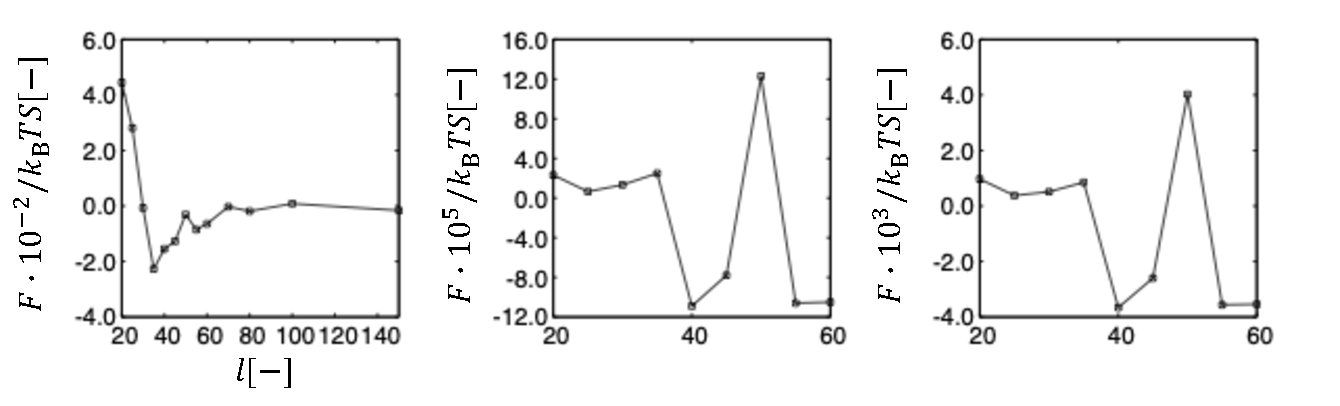
\includegraphics[width=160mm]{Fig/Fig.14/Free_Ene1.pdf}
 \put(-410,145){(a)} 
 \put(-275,145){(b)}
 \put(-120,145){(c)}
\caption{コロイド表面間の距離の関数としての(a)$\tilde{F}_{\rm{total}}$\ (b)$\tilde{F}_{\chi}$\ (c)$\tilde{F}_{\omega}$}
\label{Fig3-3-3-1}
\end{figure}
%
%\vspace{-30mm}
\begin{figure}[H]
\centering
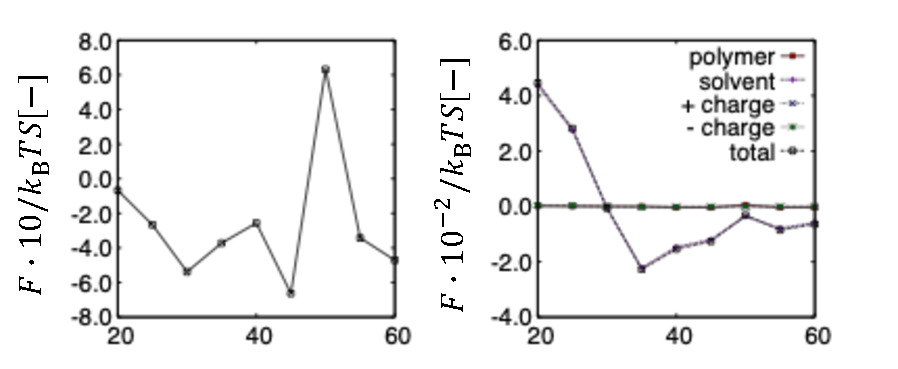
\includegraphics[width=115mm]{Fig/Fig.15/Free_Ene2.pdf}
  \put(-300,140){(d)} 
 \put(-150,140){(e)}
\caption{(d)$\tilde{F}_{e}$\ (e)$\tilde{F}_{S}$}
\label{Fig3-3-3-2}
\end{figure}
%
%\vspace{-30mm}
\begin{figure}[h]
\centering
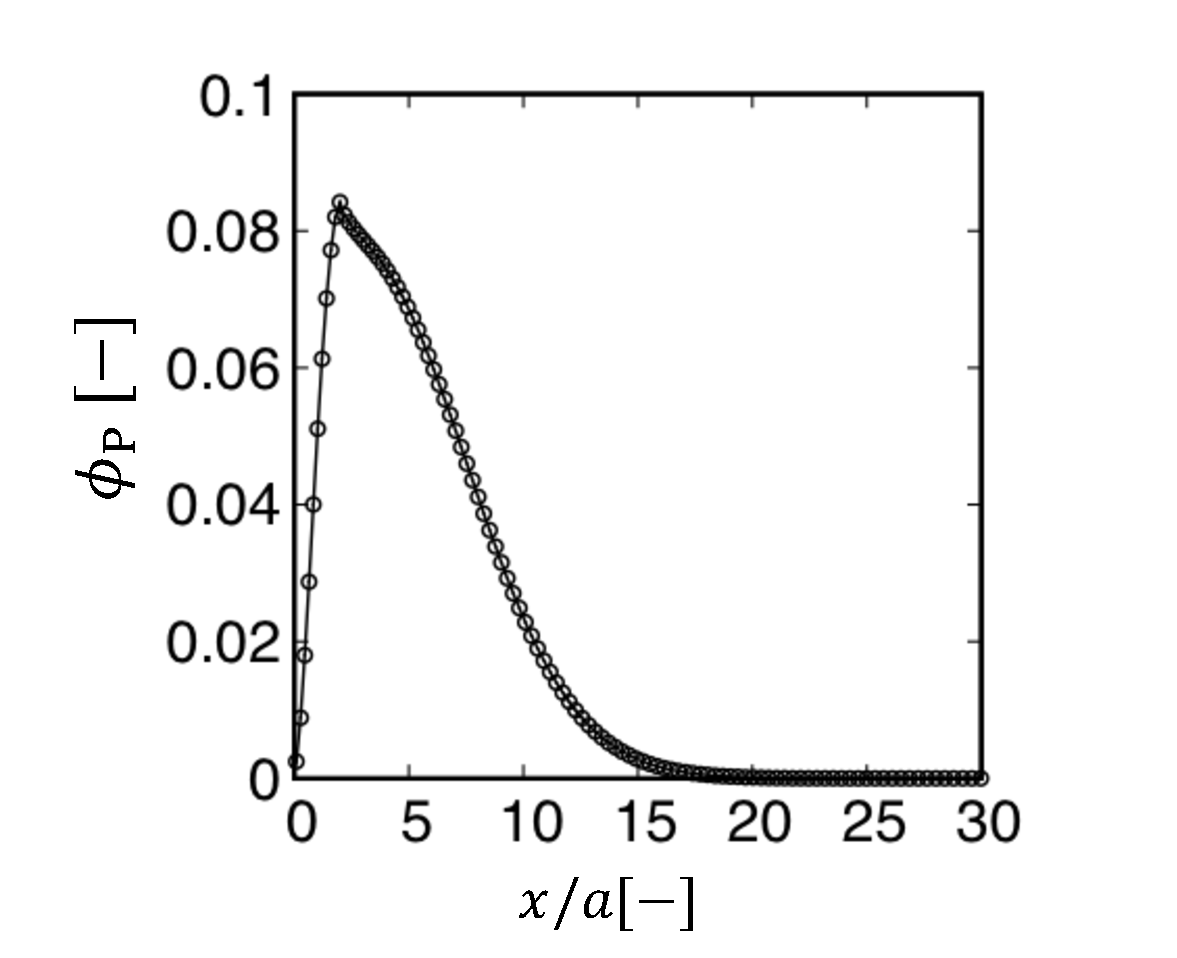
\includegraphics[width=80mm]{Fig/Fig.16/1D.pdf}
\caption{同条件下でコロイドが1つの場合の高分子ブラシセグメントの体積分率の分布}
\label{Fig3-3-4}
\end{figure}
%
%

%%%%%%%%%%%%%%%%%%%%%%%%%%%%%%%%%%%%%
%%%%%%%%%%%%%%%%%%%%%%%%%%%%%%%%%%%%%

\clearpage
\newpage
\section{結言}
%%%%%%%%%%%%%%%%%%%%%%%%%%%%%%%%%%%%%
%%%%%%%%%%%%%%%%%%%%%%%%%%%%%%%%%%%%%
\subsection{まとめ}
%%%%%%%%%%%%%%%%%%%%%%%%%%%%%%%%%%%%%
コロイド表面が平坦とみなせる場合で,電離した高分子ブラシの平衡構造を調べ,正電荷によって働く浸透圧と高分子ブラシの広がりの関係を調べた.座標系としてBispherical Coordinate System(BispC)を導入した.これにより,コロイド半径が高分子ブラシの回転慣性半径と同程度の場合を考えることが可能となり,また,コロイド間相互作用をより適切にシミュレーションすることが可能となった.また,コロイド表面を平坦とみなし,1次元でシミュレーションした結果とBispCでのシミュレーション結果を比較することで,曲率を考慮すべきコロイド半径と高分子ブラシの回転慣性半径の比の領域がわかった.コロイド間距離を変化させた際の自由エネルギーの変化から,コロイド間に働く力を考察し,両コロイドの分布範囲が重なるようなコロイド間距離で斥力が働き始めることがわかった.実際に分散安定性が保証できるほどの斥力であるかは,実験結果との定量的な比較が必要である.また,自由エネルギーの変化は溶媒のエントロピーによるエネルギー変化が支配的であることがわかった.
%%%%%%%%%%%%%%%%%%%%%%%%%%%%%%%%%%%%%
\subsection{今後の課題}
%%%%%%%%%%%%%%%%%%%%%%%%%%%%%%%%%%%%%
本研究では,シミュレーション結果に対して,定性的な考察のみを行ったが,実験結果と比較することで定量的な考察を行い,シミュレーション結果の妥当性について議論する必要がある.また,BispCでのシミュレーションにおいて,コロイド表面近傍のメッシュの大きさが位置によって異なる.このことから,コロイド表面からある微小厚み$\delta_{\rm{s}}$に対して,グラフト鎖の統計的重率の初期値$q(0,a\le r\leq a+\delta_s)=1$を与えることした.$\delta_{\rm{s}}$は$2a~3a$を与えた.課題としては,この微小厚みを極力小さくすることである.そのためには,コロイド表面近傍でメッシュを小さくするような手法を導入する必要がある.過去の研究では,コロイド半径が高分子ブラシの回転慣性半径よりも十分に大きい場合をシミュレーションしており,今回は同程度である場合をシミュレーションした.そこで,コロイド半径が高分子ブラシの回転慣性半径よりも小さい場合もシミュレーションし,他の二つの状況との比較を行う必要があると考える.また,本研究では,1種類の条件で自由エネルギーの考察を行ったが,様々な条件における自由エネルギーの考察を行うことで,より分散安定性を達成することができる条件を調べることができると考えられる.
%%%%%%%%%%%%%%%%%%%%%%%%%%%%%%%%%%%%%
\newpage
%%%%%%%%%%%%%%%%%%%%%%%%%%%%%%%%%%%%%
%%%%%%%%%%%%%%%%%%%%%%%%%%%%%%%%%%%%%
\begin{thebibliography}{99}
    \bibitem{paper1}  T. Taniguchi, {\it J. Phys. Soc. Jpn}, {\bf 78}, 041009 (2009).
    \bibitem{paper2}  M.\:Kato,  {\it{Bachelor Thesis}}, Department of Chemical Engineering, Kyoto University, (2010).

    \bibitem{paper3}  https://www.semanticscholar.org.    
    \bibitem{paper4}  Max Schelling {\it{Bachelor Thesis}}, Department of Chemical Engineering and Chemistry, Eindhoven University of Technology (2018).
    \bibitem{paper5} Q.\:Wang, T.\:Taniguchi, G.\:H.\:Fredrickson, {\it J. Phys. Soc. Chem. B}, {\bf 108}, 6733 (2004).
    \end{thebibliography}
%%%%%%%%%%%%%%%%%%%%%%%%%%%%%%%%%%%%%
%%%%%%%%%%%%%%%%%%%%%%%%%%%%%%%%%%%%%
%%%%%%%%%%%%%%%%%%%%%%%%%%%%%%%%%%%%%
\newpage
%%%%%%%%%%%%%%%%%%%%%%%%%%%%%%%%%%%%%
\pagestyle{plain}
%%%%%%%%%%%%%%%%%%%%%%%%%%%%%%%%%%%%%
\section{謝辞}
%%%%%%%%%%%%%%%%%%%%%%%%%%%%%%%%%%%%%
本研究を行うにあたり,多くの方からアドバイスやご指導をいただきました.この場を借りて感謝申し上げます.
特に,谷口先生には研究のディスカッションを初め,要旨や発表内容の添削などで親切かつ熱心にご指導いただきました.思うように研究が進まず,ディスカッションでは的外れなことを言うことも多かったと思いますが,そのような時でも,懇切丁寧にご指導いただき感謝しております.要旨や発表資料においても,私の拙い文書を添削いただきました.
先生のご指導があったからこそ,研究を終えることができました.本当にありがとうございました.\\
また,研究室内の発表にてご指導いただいた山本先生,Simonさん,Johnさん,Federicoさん,多羅間さん,瀬戸さんに深く御礼申し上げます.\\
先輩,同期の学生の皆さんには,公私共にお世話になりました.
特に,博士である佐藤さんには研究に関することを初め,多くのことを教えていただきました.感謝しています.M2の小栗さん,馬場さん,松田さん,笹倉さん,土岸さんにも感謝しております.研究に関することや,スライドの体裁など,多くの助言をいただきました.ありがとうございました.M1のBIXIAOさん,瀬領さん,玉造さん,養田さん,濱田さん,山口さんにも感謝しています.席が近いこともあり,研究で困ったことがあるときは,すぐに相談や質問をさせていただきました.ありがとうございました.また,同期の江里口君,川崎君,川角君,平松君,堀米君,南君,ありがとうございました.とても個性的な面々で,同期と過ごした研究室での日々がいい刺激となりました.

1講座の皆さんのおかげで,楽しく1年を終えることができました.大学院でも1講座を志望しているので,これからもよろしくお願いします.
%%%%%%%%%%%%%%%%%%%%%%%%%%%%%%%%%%%%%%%%%%%%%%%%%%%%%%%%%%%%%%%%%%%%%%%%%%

\end{document}
